\documentclass[10pt,a4paper]{article}
\usepackage[UTF8,fontset = windows]{ctex}
\setCJKmainfont[BoldFont=黑体,ItalicFont=楷体]{华文中宋}
\usepackage{amssymb,amsmath,amsfonts,amsthm,mathrsfs,dsfont,graphicx}
\usepackage{ifthen,indentfirst,enumerate,color,titletoc}
\usepackage{tikz}
\usepackage{multicol}
\usepackage{makecell}
\usepackage{longtable}
\usetikzlibrary{arrows,calc,intersections,patterns,decorations.pathreplacing,3d,angles}
\usepackage[bf,small,indentafter,pagestyles]{titlesec}
\usepackage[top=1in, bottom=1in,left=0.8in,right=0.8in]{geometry}
\renewcommand{\baselinestretch}{1.65}
\newtheorem{defi}{定义~}
\newtheorem{eg}{例~}
\newtheorem{ex}{~}
\newtheorem{rem}{注~}
\newtheorem{thm}{定理~}
\newtheorem{coro}{推论~}
\newtheorem{axiom}{公理~}
\newtheorem{prop}{性质~}
\newcommand{\blank}[1]{\underline{\hbox to #1pt{}}}
\newcommand{\bracket}[1]{(\hbox to #1pt{})}
\newcommand{\onech}[4]{\par\begin{tabular}{p{.9\textwidth}}
A.~#1\\
B.~#2\\
C.~#3\\
D.~#4
\end{tabular}}
\newcommand{\twoch}[4]{\par\begin{tabular}{p{.46\textwidth}p{.46\textwidth}}
A.~#1& B.~#2\\
C.~#3& D.~#4
\end{tabular}}
\newcommand{\vartwoch}[4]{\par\begin{tabular}{p{.46\textwidth}p{.46\textwidth}}
(1)~#1& (2)~#2\\
(3)~#3& (4)~#4
\end{tabular}}
\newcommand{\fourch}[4]{\par\begin{tabular}{p{.23\textwidth}p{.23\textwidth}p{.23\textwidth}p{.23\textwidth}}
A.~#1 &B.~#2& C.~#3& D.~#4
\end{tabular}}
\newcommand{\varfourch}[4]{\par\begin{tabular}{p{.23\textwidth}p{.23\textwidth}p{.23\textwidth}p{.23\textwidth}}
(1)~#1 &(2)~#2& (3)~#3& (4)~#4
\end{tabular}}

\begin{document}
\begin{enumerate}[1.]

\item 用集合语言表示下列语句并画图表示:\\
(1) 点$M$是平面$\alpha$与平面$\beta$的公共点;\\
(2) 平面$\alpha$与平面$\beta$没有公共点, 且直线$l$与平面$\alpha$和平面$\beta$分别交于点$A$和点$B$;\\
(3) 平面$\alpha$与平面$\beta$交于直线$l$, 且直线$l$与平面$\gamma$没有公共点.
\item 已知$A\in l$, $B\in l$, $Q\notin l$, 求证: 直线$OA$、$OB$、$OC$在同一平面上.
\begin{center}
    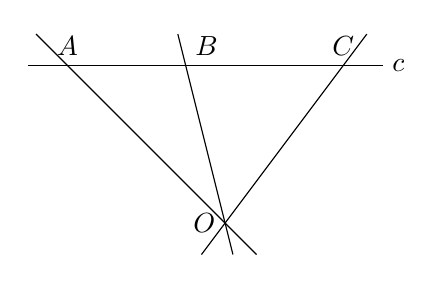
\begin{tikzpicture}
        \draw (0,0) node [left] {$O$} coordinate (O);
        \draw (-2,2) node [above] {$A$} coordinate (A);
        \draw (-0.5,2) node [above right] {$B$} coordinate (B);
        \draw (1.5,2) node [above] {$C$} coordinate (C);
        \draw (-2.5,2) -- (2,2) node [right] {$c$};
        \draw ($(O)!-0.2!(A)$) -- ($(O)!1.2!(A)$);
        \draw ($(O)!-0.2!(B)$) -- ($(O)!1.2!(B)$);
        \draw ($(O)!-0.2!(C)$) -- ($(O)!1.2!(C)$);
    \end{tikzpicture}
\end{center}
\item 判断题: (下列语句中, 正确的在横线上填入``$\checkmark$''; 错误的在横线上填入``$\times$'')\\
(1) 如果一条直线与另两条直线都相交, 那么这三条直线必共面. \blank{20};\\
(2) 如果三条直线两两都相交, 那么它们能确定一个平面. \blank{20};\\
(3) 如果三条直线相互平行, 那么这三条直线在同一个平面上. \blank{20};\\
(4) 如果两个平面都有无数个公共点, 那么这两个平面重合.   \blank{20}.
\item 过空间任意一点引四条直线, 最多可以确定几个平面? 为什么?
\item (操作探究)试用两根细绳检验一把椅子的四条腿的底端是否在同一平面内, 并说明理由.
\item 用集合语言表示下列语句并画图:
如果平面$\alpha$与平面$\beta$交于直线$l$, 平面$\alpha$与平面$\gamma$交于直线$n$, 平面$\beta$与平面$\gamma$交于直线$n$, 且直线$l$与直线$m$平行, 那么直线$l$、$m$、$n$两两平行.
\item 三个平面最多把空间分割成几个部分? 并画图表示.
\item 已知$A$、$B$、$C$、$D$、$E$是空间的五个点, 且线段$CE$、$AC$和$BD$两两相交, 求证: $A$、$B$、$C$、$D$、$E$这五个点在同一平面上.
\item 在长方体$ABCD-A_1B_1C_1D_1$中, $P$为$CC_1$上一点, 试过点$P$画棱$AD$的平行线, 并说明画法和理由.
\begin{center}
    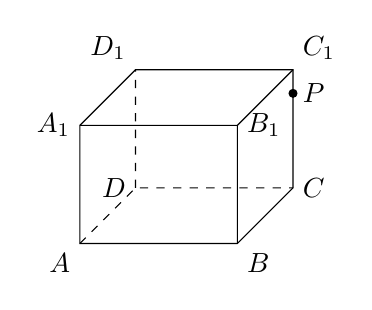
\begin{tikzpicture}
        \draw (0,0) node [below left] {$A$} coordinate (A) --++ (2,0) node [below right] {$B$} coordinate (B) --++ (45:{2/2}) node [right] {$C$} coordinate (C)
        --++ (0,1.5) node [above right] {$C_1$} coordinate (C1)
        --++ (-2,0) node [above left] {$D_1$} coordinate (D1) --++ (225:{2/2}) node [left] {$A_1$} coordinate (A1) -- cycle;
        \draw (A) ++ (2,1.5) node [right] {$B_1$} coordinate (B1) -- (B) (B1) --++ (45:{2/2}) (B1) --++ (-2,0);
        \draw [dashed] (A) --++ (45:{2/2}) node [left] {$D$} coordinate (D) --++ (2,0) (D) --++ (0,1.5);
        \filldraw ($(C)!0.8!(C1)$) circle (0.05) node [right] {$P$};
    \end{tikzpicture}
\end{center}
\item 在空间四边形$ABCD$中, $E,F,G,H$分别是$AB,BC,CD,DA$的中点, 且$AC=BD$, 试证明$EFGH$是平面图形, 并分析四边形$EFGH$的性质.
\begin{center}
    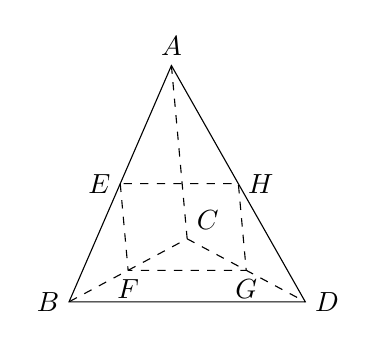
\begin{tikzpicture}
        \draw (0,0) node [left] {$B$} coordinate (B);
        \draw (3,0) node [right] {$D$} coordinate (D);
        \draw (1.3,3) node [above] {$A$} coordinate (A);
        \draw (1.5,0.8) node [above right] {$C$} coordinate (C);
        \draw ($(A)!0.5!(B)$) node [left] {$E$} coordinate (E);
        \draw ($(B)!0.5!(C)$) node [below] {$F$} coordinate (F);
        \draw ($(C)!0.5!(D)$) node [below] {$G$} coordinate (G);
        \draw ($(D)!0.5!(A)$) node [right] {$H$} coordinate (H);
        \draw (A) -- (B) -- (D) -- cycle;
        \draw [dashed] (A) -- (C) -- (B) (C) -- (D);
        \draw [dashed] (E) -- (F) -- (G) -- (H) -- cycle;
    \end{tikzpicture}
\end{center}
\item 如图, 在正方体$ABCD-A_1B_1C_1D_1$中$O_1$、$O_2$分别是正方形$ABB_1A_1$, 和正方形$DCC_1D_1$的对角线的交点, 求证: $\angle A_1O_1D_1=\angle CO_2B$.
\begin{center}
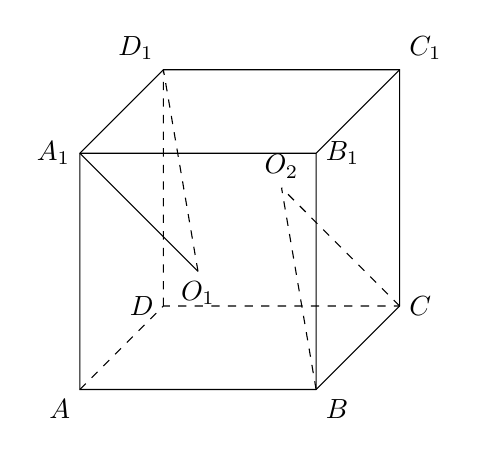
\begin{tikzpicture}[>=latex,scale = 1.5]
\draw (0,0) node [below left] {$A$} coordinate (A) --++ (2,0) node [below right] {$B$} coordinate (B) --++ (45:{2/2}) node [right] {$C$} coordinate (C)
--++ (0,2) node [above right] {$C_1$} coordinate (C1)
--++ (-2,0) node [above left] {$D_1$} coordinate (D1) --++ (225:{2/2}) node [left] {$A_1$} coordinate (A1) -- cycle;
\draw (A) ++ (2,2) node [right] {$B_1$} coordinate (B1) -- (B) (B1) --++ (45:{2/2}) (B1) --++ (-2,0);
\draw [dashed] (A) --++ (45:{2/2}) node [left] {$D$} coordinate (D) --++ (2,0) (D) --++ (0,2);
\draw ($(C)!0.5!(D1)$) node [above] {$O_2$} coordinate (O2);
\draw ($(B)!0.5!(A1)$) node [below] {$O_1$} coordinate (O1);
\draw (A1) -- (O1);
\draw [dashed] (O1) -- (D1) (B) -- (O2) (C) -- (O2);
\end{tikzpicture}
\end{center}
\item 在长方体$ABCD-A_1B_1C_1D_1$中, $P,Q$分别为$CC_1AA_1$的中点, 求证: $BP\parallel D_1Q$.
\begin{center}
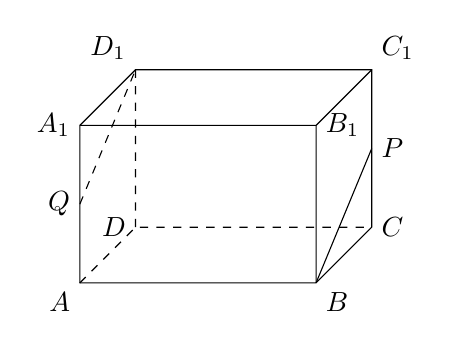
\begin{tikzpicture}[>=latex]
\draw (0,0) node [below left] {$A$} coordinate (A) --++ (3,0) node [below right] {$B$} coordinate (B) --++ (45:{2/2}) node [right] {$C$} coordinate (C)
--++ (0,2) node [above right] {$C_1$} coordinate (C1)
--++ (-3,0) node [above left] {$D_1$} coordinate (D1) --++ (225:{2/2}) node [left] {$A_1$} coordinate (A1) -- cycle;
\draw (A) ++ (3,2) node [right] {$B_1$} coordinate (B1) -- (B) (B1) --++ (45:{2/2}) (B1) --++ (-3,0);
\draw [dashed] (A) --++ (45:{2/2}) node [left] {$D$} coordinate (D) --++ (3,0) (D) --++ (0,2);
\draw ($(C)!0.5!(C1)$) node [right] {$P$} -- (B);
\draw [dashed] ($(A)!0.5!(A1)$) node [left] {$Q$} -- (D1);
\end{tikzpicture}
\end{center}
\item 证明公理$3$的推论$3$.
\item 已知直线$l$上有$ABC$三点, 过这三点分别作三条互相平行$abc$直线. 求证: $l,a,b,c$四条直线都在同一平面内.
\begin{center}
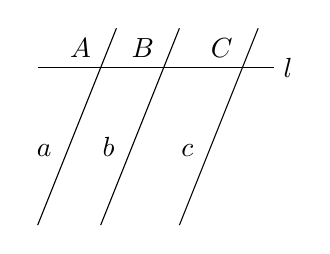
\begin{tikzpicture}[>=latex]
\draw (0,0) -- (3,0) node [right] {$l$};
\draw (0,-2) coordinate (A1) -- (1,0.5) coordinate (A2);
\draw (0.8,-2) coordinate (B1) -- (1.8,0.5) coordinate (B2);
\draw (1.8,-2) coordinate (C1) -- (2.8,0.5) coordinate (C2);
\draw ($(A1)!0.8!(A2)$) node [above left] {$A$} ($(A1)!0.3!(A2)$) node [above left] {$a$};
\draw ($(B1)!0.8!(B2)$) node [above left] {$B$} ($(B1)!0.3!(B2)$) node [above left] {$b$};
\draw ($(C1)!0.8!(C2)$) node [above left] {$C$} ($(C1)!0.3!(C2)$) node [above left] {$c$};
\end{tikzpicture}
\end{center}
\item 已知$ABCD$是不共面的四个点, 证明: 直线$AB$与$CD$是异面直线.
\item 在正方体$ABCD-A_1B_1C_1D_1$中, $AC$与$DB$交于点$O$, $B_1O$与$AA_1$是不是异面直线? 为什么?
\item 在正方体$ABCD-A'B'C'D'$中, $P,Q$分别为$A'B',BB'$的中点.\\
(1) 求直线$AP$与$CQ$所成的角的大小;\\
(2) 求直线$AP$与$BD$所成的角的大小.
\item 已知点$P$在四边形$ABCD$所在乎面外, 如果把两条异面直线看成一对. 那么$P$与四边形$ABCD$的四个顶点的连线以及此四边形的四条边所在的直线共$8$条直线中, 异面直线共有多少对?
\item 已知正方体$ABCD-A_1B_1C_1D_1$中, $E,F,G,H$分别是棱$AB,BC,C_1D_1,A_1D_1$的中点, 求证: 点$E,F,G,H$在同一平面内.
\begin{center}
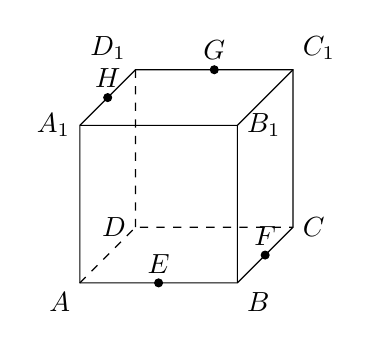
\begin{tikzpicture}[>=latex]
\draw (0,0) node [below left] {$A$} coordinate (A) --++ (2,0) node [below right] {$B$} coordinate (B) --++ (45:{2/2}) node [right] {$C$} coordinate (C)
--++ (0,2) node [above right] {$C_1$} coordinate (C1)
--++ (-2,0) node [above left] {$D_1$} coordinate (D1) --++ (225:{2/2}) node [left] {$A_1$} coordinate (A1) -- cycle;
\draw (A) ++ (2,2) node [right] {$B_1$} coordinate (B1) -- (B) (B1) --++ (45:{2/2}) (B1) --++ (-2,0);
\draw [dashed] (A) --++ (45:{2/2}) node [left] {$D$} coordinate (D) --++ (2,0) (D) --++ (0,2);
\filldraw ($(A)!0.5!(B)$) circle (0.05) node [above] {$E$};
\filldraw ($(C)!0.5!(B)$) circle (0.05) node [above] {$F$};
\filldraw ($(C1)!0.5!(D1)$) circle (0.05) node [above] {$G$};
\filldraw ($(A1)!0.5!(D1)$) circle (0.05) node [above] {$H$};
\end{tikzpicture}
\end{center}
\item 在长方体$ABCD-A_1B_1C_1D_1$中, $E,F$分别是棱$A_1,B_1,D,C$的点, 且$EB_1=DF$, 求证: $\triangle AED_1\cong \triangle C_1FB$.
\begin{center}
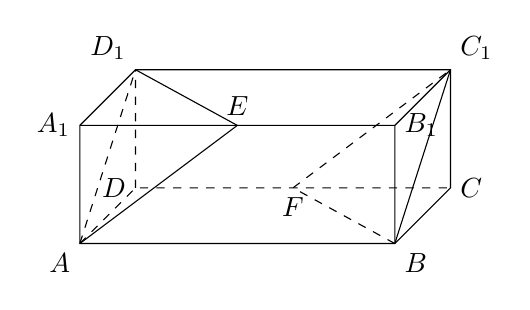
\begin{tikzpicture}[>=latex]
\draw (0,0) node [below left] {$A$} coordinate (A) --++ (4,0) node [below right] {$B$} coordinate (B) --++ (45:{2/2}) node [right] {$C$} coordinate (C)
--++ (0,1.5) node [above right] {$C_1$} coordinate (C1)
--++ (-4,0) node [above left] {$D_1$} coordinate (D1) --++ (225:{2/2}) node [left] {$A_1$} coordinate (A1) -- cycle;
\draw (A) ++ (4,1.5) node [right] {$B_1$} coordinate (B1) -- (B) (B1) --++ (45:{2/2}) (B1) --++ (-4,0);
\draw [dashed] (A) --++ (45:{2/2}) node [left] {$D$} coordinate (D) --++ (4,0) (D) --++ (0,1.5);
\draw ($(A1)!0.5!(B1)$) node [above] {$E$} coordinate (E);
\draw ($(C)!0.5!(D)$) node [below] {$F$} coordinate (F);
\draw (D1) -- (E) -- (A) (B) -- (C1);
\draw [dashed] (A) -- (D1) (B) -- (F) -- (C1);
\end{tikzpicture}
\end{center}
\item 已知直线$c,d$分别与异面直线$a,b$相交于$E,F$和$G,H$四个两两不重合的点, 求证: 直线$c,d$是异面直线.
\item 在正方体$ABCD-A_1B_1C_1D_1$中, $EF$分别是$BDB_1C$上的点, 且$BE=B_1F=\dfrac 23B_1C$, 求直线$EF$与$CD$所成的角的大小.
\begin{center}
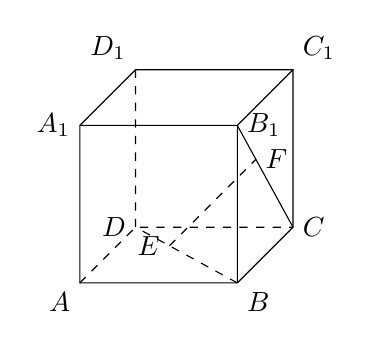
\begin{tikzpicture}[>=latex]
\draw (0,0) node [below left] {$A$} coordinate (A) --++ (2,0) node [below right] {$B$} coordinate (B) --++ (45:{2/2}) node [right] {$C$} coordinate (C)
--++ (0,2) node [above right] {$C_1$} coordinate (C1)
--++ (-2,0) node [above left] {$D_1$} coordinate (D1) --++ (225:{2/2}) node [left] {$A_1$} coordinate (A1) -- cycle;
\draw (A) ++ (2,2) node [right] {$B_1$} coordinate (B1) -- (B) (B1) --++ (45:{2/2}) (B1) --++ (-2,0);
\draw [dashed] (A) --++ (45:{2/2}) node [left] {$D$} coordinate (D) --++ (2,0) (D) --++ (0,2);
\draw [dashed] ($(B)!{2/3}!(D)$) node [left] {$E$} -- ($(C)!{2/3}!(B1)$) node [right] {$F$};
\draw (C) -- (B1);
\draw [dashed] (B) -- (D);
\end{tikzpicture}
\end{center}
\item ``直线$l$垂直于平面$\alpha$内的无数条直线''是``$l\perp \alpha$''的\blank{50}条件. (填``充分''或``必要``或``充要''或``既非充分又非必要'')
\item 在正方体$ABCD-A_1B_1C_1D_1$中找出表示下列距离的线段:
\begin{center}
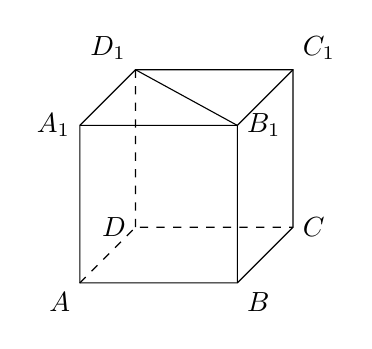
\begin{tikzpicture}[>=latex]
\draw (0,0) node [below left] {$A$} coordinate (A) --++ (2,0) node [below right] {$B$} coordinate (B) --++ (45:{2/2}) node [right] {$C$} coordinate (C)
--++ (0,2) node [above right] {$C_1$} coordinate (C1)
--++ (-2,0) node [above left] {$D_1$} coordinate (D1) --++ (225:{2/2}) node [left] {$A_1$} coordinate (A1) -- cycle;
\draw (A) ++ (2,2) node [right] {$B_1$} coordinate (B1) -- (B) (B1) --++ (45:{2/2}) (B1) --++ (-2,0);
\draw [dashed] (A) --++ (45:{2/2}) node [left] {$D$} coordinate (D) --++ (2,0) (D) --++ (0,2);
\draw (B1) -- (D1);
\end{tikzpicture}
\end{center}
(1) 点$A$, 到直线$BC$的距离为\blank{50};\\
(2) 点$A$到平面$B_1BCC_1$的距离为\blank{50};\\
(3) $B_1D_1$和平面$ABCD$的距离为\blank{50}.
\item 在长方体$ABCD-A_1B_1C_1D_1$中, 找出下列异面直线的公垂线段.
\begin{center}
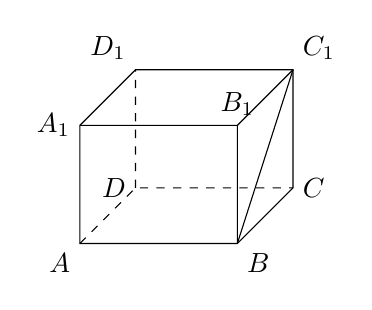
\begin{tikzpicture}[>=latex]
\draw (0,0) node [below left] {$A$} coordinate (A) --++ (2,0) node [below right] {$B$} coordinate (B) --++ (45:{2/2}) node [right] {$C$} coordinate (C)
--++ (0,1.5) node [above right] {$C_1$} coordinate (C1)
--++ (-2,0) node [above left] {$D_1$} coordinate (D1) --++ (225:{2/2}) node [left] {$A_1$} coordinate (A1) -- cycle;
\draw (A) ++ (2,1.5) node [above] {$B_1$} coordinate (B1) -- (B) (B1) --++ (45:{2/2}) (B1) --++ (-2,0);
\draw [dashed] (A) --++ (45:{2/2}) node [left] {$D$} coordinate (D) --++ (2,0) (D) --++ (0,1.5);
\draw (B) -- (C1);
\end{tikzpicture}
\end{center}
(1) $AB$和$DD_1$;\\
(2) $AA_1$和$BC_1$.
\item 有一根旗杆$AB$高$8$米, 它的顶端挂一条长$10$米的绳子, 拉紧绳子并把它的下端放在地面上的两点(和旗杆脚不在同一直线上) $C$、$D$. 如果这两个点和旗杆脚$B$的距离都是$6$米, 那么旗杆就和地面垂直, 为什么?
\item 判断题: (下列命题中, 是真命题的在横线上填入``$\checkmark$''; 是假命题的在横线上填入``$\times$'')\\
(1) 一条直线在平面内的射影是一条直线.\blank{20};\\
(2) 在平面内射影是直线的图形一定是直线.\blank{20};\\
(3) 如果两条线段在同一平面内的射影长相等, 那么这两条线段的长相等.\blank{20};\\
(4) 如果两条斜线与平面所成的角相等, 那么这两条斜线互相平行.\blank{20}.
\item 过平面$\alpha$外一点$P$的斜线段$PA$的长是过这点的垂线段$PB$的$\dfrac{2\sqrt 3}3$倍$(AB\in \alpha) $, 求斜线$PA$与平面$\alpha$所成的角的大小.
\item 已知$\triangle ABC$, 点$P$是平面$ABC$外一点, 点$O$是点$P$在平面$ABC$上的射影, 且点$O$在$\triangle ABC$内.
\item 若点$P$到$\triangle ABC$的三个顶点的距离相等, 则点$O$一定是$\triangle ABC$\blank{50}心.
\item 若点$P$到$\triangle ABC$的三边所在直线的距离相等, 则点$O$一定是$\triangle ABC$的\blank{50}心.
\item 在长方体$ABCD-A_1B_1C_1D_1$中, $AB=BC=4$, $A_1A=5$, $M$是$AB$的中点. 求直线$C_1M$与平面$ABCD$所成的角的大小.
\begin{center}
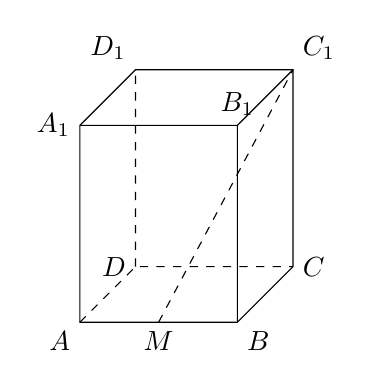
\begin{tikzpicture}[>=latex]
\draw (0,0) node [below left] {$A$} coordinate (A) --++ (2,0) node [below right] {$B$} coordinate (B) --++ (45:{2/2}) node [right] {$C$} coordinate (C)
--++ (0,2.5) node [above right] {$C_1$} coordinate (C1)
--++ (-2,0) node [above left] {$D_1$} coordinate (D1) --++ (225:{2/2}) node [left] {$A_1$} coordinate (A1) -- cycle;
\draw (A) ++ (2,2.5) node [above] {$B_1$} coordinate (B1) -- (B) (B1) --++ (45:{2/2}) (B1) --++ (-2,0);
\draw [dashed] (A) --++ (45:{2/2}) node [left] {$D$} coordinate (D) --++ (2,0) (D) --++ (0,2.5);
\draw [dashed] ($(A)!0.5!(B)$) node [below] {$M$} -- (C1);
\end{tikzpicture}
\end{center}
\item 如果三个平面两两相交于三条直线, 请指出这三条直线的位置关系, 并说明理由.
\item 如图, $EF$分别是空间四边形$ABCD$的边$BCAD$的中点, 过$EF$且平行于$AB$的平面与$AC$交于点$G$, 求证: $G$是$AC$的中点.
\begin{center}
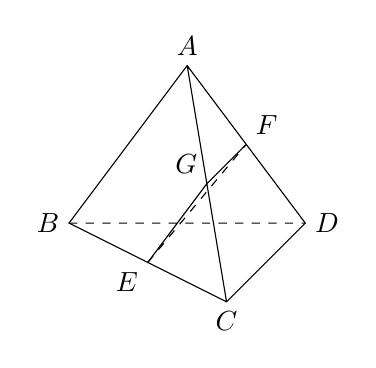
\begin{tikzpicture}[>=latex]
\draw (0,0) node [left] {$B$} coordinate (B);
\draw (3,0) node [right] {$D$} coordinate (D);
\draw (2,-1) node [below] {$C$} coordinate (C);
\draw (1.5,2) node [above] {$A$} coordinate (A);
\draw ($(B)!0.5!(C)$) node [below left] {$E$} coordinate (E);
\draw ($(A)!0.5!(D)$) node [above right] {$F$} coordinate (F);
\draw ($(A)!0.5!(C)$) node [above left] {$G$} coordinate (G);
\draw (A) -- (B) -- (C) -- (D) -- cycle (A) -- (C) (E) -- (G) -- (F);
\draw [dashed] (E) -- (F) (B) -- (D);
\end{tikzpicture}
\end{center}
\item 在长方体$ABCD-A_1B_1C_1D_1$中, 矩形$AA_1D_1D$和$D_1C_1CD$的中心分别为$MN$, 求证: $MN\parallel$平面$ABCD$.
\begin{center}
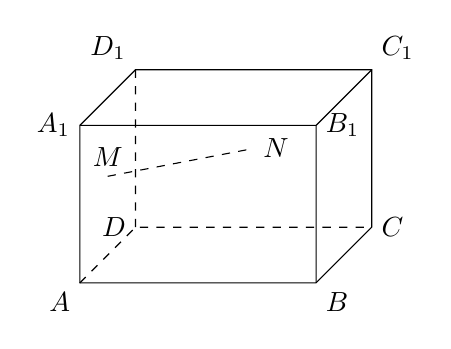
\begin{tikzpicture}[>=latex]
\draw (0,0) node [below left] {$A$} coordinate (A) --++ (3,0) node [below right] {$B$} coordinate (B) --++ (45:{2/2}) node [right] {$C$} coordinate (C)
--++ (0,2
) node [above right] {$C_1$} coordinate (C1)
--++ (-3,0) node [above left] {$D_1$} coordinate (D1) --++ (225:{2/2}) node [left] {$A_1$} coordinate (A1) -- cycle;
\draw (A) ++ (3,2
) node [right] {$B_1$} coordinate (B1) -- (B) (B1) --++ (45:{2/2}) (B1) --++ (-3,0);
\draw [dashed] (A) --++ (45:{2/2}) node [left] {$D$} coordinate (D) --++ (3,0) (D) --++ (0,2
);
\draw [dashed] ($(A)!0.5!(D1)$) node [above] {$M$} -- ($(C)!0.5!(D1)$) node [right] {$N$}; 
\end{tikzpicture}
\end{center}
\item 在空间四边形$ABCD$中, $AB=DC=4$, $BC=AD=3$, $AD\perp BC$, $AB\perp BC$.\\
(1) 求证: $BD$是$AD$、$BC$的公垂线;\\
(2) 求$BD$的长.
\item 已知正方体$ABCD-A_1B_1C_1D_1$的棱长为$1$.\\
(1) 点$A$到$CD_1$的距离为\blank{50};\\
(2) 点$A$到$BD_1$的距离为\blank{50};\\
(3) 点$A$到面$BB_1D_1D$的距离为\blank{50};\\
(4) $AA_1$和面$BB_1D_1D$的距离为\blank{50}.
(第2题)
\item 已知$P$是等边三角形$ABC$所在平面外一点, $PA=PB=PC=\dfrac 23$, $\triangle ABC$的边长为$1$. 求$PC$和平面$ABC$所成的角的大小.
\item $PA, PB$是平面$\alpha$的斜线, 已知$\angle APB=90^\circ$, $AB=10$, 点$P$到平面$\alpha$的距离为$3$, $PA$和平面$\alpha$所成的角为$30^\circ$. 求平面$\alpha$所成的角的大小.
\item 已知$ABCD$是不共面的四个点, $M,N$分别是$\triangle ACD,\triangle BCD$的重心. 试判断平面$ABC$, 平面$ACD$、平面$BCD$中, 哪些平面与$MN$平行, 并说明理由.
\item 判断题: (下列命题中, 是真命题的在横线上填入``$\checkmark$''; 是假命题的在横线上填入``$\times$'')\\
(1) 二面角指的是两个平面相交所组成的图形.\blank{20};\\
(2) 二面角指的是一个平面绕这个平面内的一条直线旋转所组成的图形.\blank{20};\\
(3) 二面角指的是以一个平面内的一条直线为边界的一个半平面与这个平面所组成的图形.\blank{20};\\
(4) 二面角指的是从一条直线出发的两个半平面所组成的图形.\blank{20}.
\item 已知二面角$\alpha -AB-\beta$为$30^\circ$, $P$是面$\alpha$内一点, 点$P$到面$\beta$的距离是$1$, 求点$P$在面$\beta$内的射影到$AB$的距离.
\item 已知$P$是二面角$\alpha -AB-\beta$内一点, $PC\perp \alpha$, 垂足为$C$, $PD\perp \beta$, 垂足为$D$, 且$PC=3$, $PD=4$, $\angle CPD=60^\circ$.\\
(1) 求二面角$\alpha -AB-\beta$的大小;\\
(2) 求$CD$的长.
\item 在正方体中$ABCD-A_1B_1C_1D_1$中, $E_1$为$A_1D_1$的中点.
\begin{center}
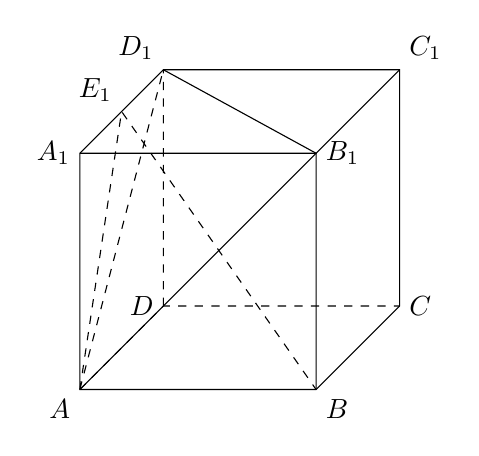
\begin{tikzpicture}[>=latex]
\draw (0,0) node [below left] {$A$} coordinate (A) --++ (3,0) node [below right] {$B$} coordinate (B) --++ (45:{3/2}) node [right] {$C$} coordinate (C)
--++ (0,3) node [above right] {$C_1$} coordinate (C1)
--++ (-3,0) node [above left] {$D_1$} coordinate (D1) --++ (225:{3/2}) node [left] {$A_1$} coordinate (A1) -- cycle;
\draw (A) ++ (3,3) node [right] {$B_1$} coordinate (B1) -- (B) (B1) --++ (45:{3/2}) (B1) --++ (-3,0);
\draw [dashed] (A) --++ (45:{3/2}) node [left] {$D$} coordinate (D) --++ (3,0) (D) --++ (0,3);
\draw ($(A1)!0.5!(D1)$) node [above left] {$E_1$} coordinate (E1);
\draw (D1) -- (B1) -- (A);
\draw [dashed] (A) -- (E1) -- (B) (A) -- (D1);
\end{tikzpicture}
\end{center}
(1) 求二面角$E_1-AB-C$的大小;\\
(2) 求二面角$C_1-B_1D_1-A$的大小.
\item 平行于同一直线的两个平面是否平行?
\item 两个平面分别经过两条平行直线, 这两个平面是否平行?
\item 分别在两个平行平面内的两条直线是否平行?
\item 选择题:
(1) $\alpha,\beta$是两个不重合的平面, $a,b$是两条不同的直线, 在下列条件中可判定$\alpha \parallel\beta$的是\bracket{20}.
\onech{平面$\alpha,\beta$都平行于直线$a,b$}{平面内有三个不共线的点到平面$\beta$的距离相等}{$a,b$是平面$\alpha$内的两条直线, 且$\alpha \parallel\beta$, $b\parallel\beta$}{$a,b$是两条异面直线, 且$a\parallel\alpha$, $b\parallel\alpha$, $\alpha \parallel\beta$, $b\parallel\beta$}
\item 下列命题中不正确的是\bracket{20}.
\onech{如果平面$\alpha$与平面$\beta$平行, 那么平面$\alpha$内任一直线平行于平面$\beta$}{如果一个平面内任何一条直线都平行于另一个平面, 那么这两个平面平行}{如果一条直线$m$与两个平面$\alpha$、$\beta$所成的角相等, 那么$\alpha \parallel\beta$}{分别在两个平行平面内的两条直线只能是平行直线或异面直线}
\item 在正方体$ABCD-A'B'C'D'$中, $E,F,G$分别是$AD,DD',DC$的中点, 求证: 平面$EFG$平行于平面$A'BC'$.
\item 某人在山坡上沿着与山坡脚线(山坡面与水平地面的交线)垂直的方向上坡, 如果每前进$200$米, 上升的高度为$50\sqrt 3$米, 求坡面与水平面所成的二面角的大小.
\item 已知边长为$\alpha$的正方形$ABCD$外有一点$P$.使$PA\perp$平面$ABCD$. $PA=a$. 求二面角$A-PB-C$和$B-PC-D$的大小.
\item 设$a,b$是异面直线, 直线$a$在平面$a$内, 直线$b$在平面$\beta$内, 且$a\parallel\beta$, $b\parallel a$, 求证: $a\parallel\beta$.
\item 已知不共面的三条直线$a,b,c$相交于点$P$, 平面$\alpha,\beta$与直线$a,b,c$分别相交于$A,B,C$和$A_1,B_1,C_1$, 且$\dfrac{PA}{PA_1}=\dfrac{PB}{PB_1}=\dfrac{PC}{PC_1}$, 求证: $\alpha \parallel\beta$.
\item 画出下列点、直线和平面之间的位置关系图, 并用集合符号表示.\\
(1) 直线$l$在平面$\alpha$上, 点$M$在平面$\alpha$上, 但不在直线$l$上;\\
(2) 平面$\alpha$与平面$\beta$交于直线$l$. 直线$a$与平面$\alpha$、平面$\beta$都没有公共点.
\item 将下列集合符号表述改为自然语言表述, 并判断它们是否正确.\\
(1) $A\in \beta$, $B\in \beta \Rightarrow AB\not\in \beta$;\\
(2) $A\in \alpha$, $B\in \alpha$, $C\in AB\Rightarrow C\in \alpha$.
\item 已知直线$AB\parallel CD$, 平面$\alpha$满足: $AB\cap \alpha =E$, $CD\cap \alpha \text=F$, 求作直线$BC$与平面$\alpha$的交点.
\item 在长方体$ABCD-A'B'C'D'$的面$A'C'$上有一点$P$, 过点$P$在面$A'C'$上画一条直线和$BD$平行, 应当如何画? 并说明理由.
\begin{center}
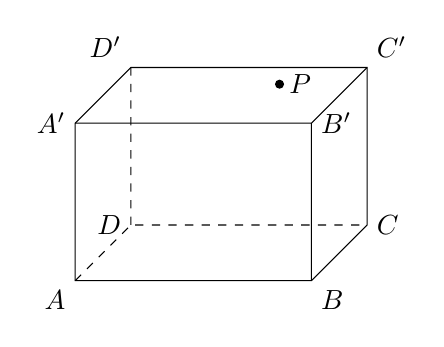
\begin{tikzpicture}[>=latex]
\draw (0,0) node [below left] {$A$} coordinate (A) --++ (3,0) node [below right] {$B$} coordinate (B) --++ (45:{2/2}) node [right] {$C$} coordinate (C)
--++ (0,2) node [above right] {$C'$} coordinate (C1)
--++ (-3,0) node [above left] {$D'$} coordinate (D1) --++ (225:{2/2}) node [left] {$A'$} coordinate (A1) -- cycle;
\draw (A) ++ (3,2) node [right] {$B'$} coordinate (B1) -- (B) (B1) --++ (45:{2/2}) (B1) --++ (-3,0);
\draw [dashed] (A) --++ (45:{2/2}) node [left] {$D$} coordinate (D) --++ (3,0) (D) --++ (0,2);
\filldraw ($(A1)!0.7!(C1)$) circle (0.05) node [right] {$P$};
\end{tikzpicture}
\end{center}
\item 回答下列问题:\\
(1) 垂直于同一直线的两个平面是否平行?\\
(2) 平行于同一平面的两条直线是否平行?\\
(3) 垂直于同一平面的两条直线是否平行?
\item 判断下列说法是否正确, 如果正确, 请说明理由; 如果不正确, 请举出反例.\\
(1) 三角形一定是平面图形;\\
(2) 一组对边平行的四边形一定是平面图形;\\
(3) 两组对边相等的四边形一定是平面图形;\\
(4) 两条不平行的直线一定是相交直线.
\item 已知$E,F,G,H$分别是空间四边形$ABCD$的各边$AB,DA,BC,CD$上的点, 且直线$EF$和$GH$交于点$P$. 求证: 点$B,D,P$在同一条直线上.
\item 在正方体$ABCD-A_1B_1C_1D_1$中, $P,Q$分别为$AB,BC$的中点. 求$PQ$与下列各直线所成的角的大小:\\
(1) $CC_1$;\\
(2) $AC_1$;\\
(3) $B_1C$.
\item 已知$AB$是平面$\alpha$外两点, $AB$到平面$\alpha$的距离分别为$2\text{cm}$、$4\text{cm}$. 且$AB$在平向$\alpha$上的射影间的距离为$6c\text{cm}$, 求线段$AB$的长.
\item 在长方体$ABCD-A_1B_1C_1D_1$中, $O,O_1$分别为四边形$ABCD$、$A_1B_1C_1D_1$中心, $E,F$分别为四边形$AA_1D_1D,BB_1C_1C$的中心, $G,H$分别为四边形$A_1ABB_1,C_1CDD_1$的中心, 求证: $\triangle OGE\cong O_1FH$.
\item 在长方体$ABCD-A_1B_1C_1D_1$中, $AB=4$, $BC=AA=3$, 分别求直线$BD_1$与平面$ABCD$、直线$BD_1$与平面$BB_1C_1C$所成的角的大小.
\item 在$\text{Rt}\triangle ABC$中, 两直角边$AC,BC$的长分别为$9$、$12$, $PC$垂直于平面$ABC$, $PC=6$, 求点$P$到斜边$AB$的距离.
\item 在空间四边形$ABCD$, $AC=BC,AD=BD$, 求证: $AB\perp CD$.
\item 在$120^\circ$的二面角的棱上有$A,B$两点, $AC,BD$分别是这个二面角的两个面内垂直于$AB$的线段, 已知: $AB=4$, $AC=6$, $BD=8$, 求$CD$的长.
\item 在正方体$ABCD-A'B'C'D'$中, $AB'$和$BC'$所成的角的大小是\bracket{20}.
\fourch{$30^\circ$}{$45^\circ$}{$60^\circ$}{$90^\circ$}
\item 若$O_1$为正方体$ABCD-A_1B_1C_1D_1$的面$A_1B_1C_1D_1$的中心, 则直线$BC_1$与对角面$BB_1D_1D$所成的角等于
\fourch{$\angle C_1BD_1$}{$\angle C_1BO_1$ }{$\angle C_1BB_1$ }{$\angle C_1BD$}
\item 如果长方体的一条对角线与过同一个顶点的三个面所成的角分别是$\alpha,\beta,\gamma$那么$\sin ^2\alpha +\sin ^2\beta +\sin ^2\gamma \text=$\blank{50}.
\item 三个平面可将空间分成\blank{50}个部分.
\item 在空间四边形$ABCD$中, $AB=BC=CD=DA=AC=BD=a$, 是$BC$的中点, 求异面直线$AC$与$DF$所成的角的大小.
\item 已知$CD$是$\alpha$、$\beta$的交线, $EA\perp \alpha$垂足为$A$, $EB\perp \beta$, 垂足为$B$. 求证: $CD\perp AB$.
\item 已知$PA$垂直于$\triangle ABC$所在的平面$\alpha$, $D$为$BC$的中点, 又$PB,PD,PC$与平面$\alpha$所成的角分别为$60^\circ$、$45^\circ$、$30^\circ$, 且$BC=6\text{cm}$, 求$PA$的长.
\item 已知$P$为平行四边形$ABCD$所在平面外一点, $M$为$PB$的中点, 求证: $PD\parallel$平面$MAC$.
\item 已知空间四边形$OABC$各边及对角线的长都是$1$, $D,E$分别是边$OA,BC$的中点, 联结$DE$.
(1) 求证: $DE$是异面直线$OA$和$BC$的公垂线段;\\
(2) 求$DE$的长;\\
(3) 求点$O$到平面$ABC$的距离.
\item 如图, 已知二面角$\alpha -l-\beta$的两个面内各有一点$AB$, $AB$在直线$l$的射影分别为点$CD$, $AC=3$, $BD=3$, 而$CD=4$, $AB=5$. 求二面角$\alpha -l-\beta$的大小.
\begin{center}
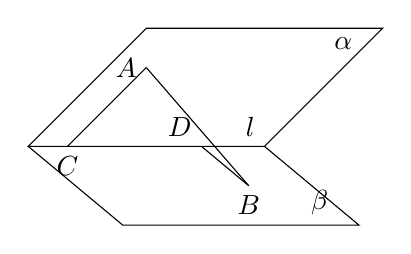
\begin{tikzpicture}[>=latex]
\draw (0,0) -- (3,0) node [above left] {$l$} -- (4.5,1.5) -- (1.5,1.5) -- cycle;
\draw (3,0) -- (4.2,-1) -- (1.2,-1) -- (0,0);
\draw (0.5,0) node [below] {$C$} --++ (1,1) node [left] {$A$} coordinate (A);
\draw (2.2,0) node [above left] {$D$} --++ (0.6,-0.5) node [below] {$B$} coordinate (B);
\draw (A) -- (B);
\draw (4,1.5) node [below] {$\alpha$};
\draw (3.7,-1) node [above] {$\beta$};
\end{tikzpicture}
\end{center}
\item 分别写出下列多面体的名称:
\begin{center}
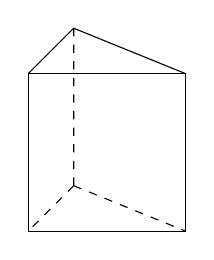
\begin{tikzpicture}[>=latex]
\draw (0,0,0) -- (2,0,0) -- (2,2,0) -- (0,2,0) -- cycle;
\draw [dashed] (0,0,-1.5) -- (0,2,-1.5) (0,0,-1.5) -- (0,0,0) (0,0,-1.5) -- (2,0,0);
\draw (0,2,0) -- (0,2,-1.5) -- (2,2,0);
\end{tikzpicture}
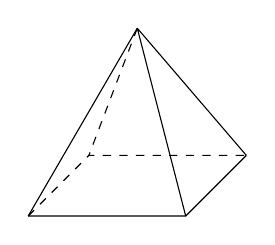
\begin{tikzpicture}
\draw (1,0,-1) -- (1,0,1) -- (-1,0,1);
\draw [dashed] (-1,0,1) -- (-1,0,-1) -- (1,0,-1);
\draw (0,2,0) -- (1,0,-1) (0,2,0) -- (1,0,1) (0,2,0) -- (-1,0,1);
\draw [dashed] (0,2,0) -- (-1,0,-1);
\end{tikzpicture}
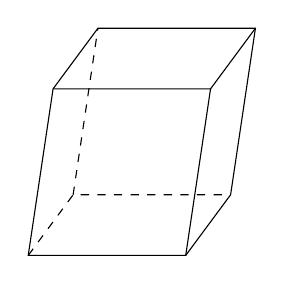
\begin{tikzpicture}
\draw (0,0,0) -- (2,0,0) --++ (-0.2,0,-2) --++ (0.2,2,-0.3) --++ (-2,0,0) --++ (0.2,0,2) -- cycle;
\draw (2,0,0) --++ (0.2,2,-0.3) --++ (-2,0,0);
\draw (2,0,0) ++ (0.2,2,-0.3) --++ (-0.2,0,-2);
\draw [dashed] (0,0,0) --++ (-0.2,0,-2) --++ (2,0,0);
\draw [dashed] (0,0,0) ++ (-0.2,0,-2) --++ (0.2,2,-0.3);
\end{tikzpicture}
\end{center}
\item 斜棱柱、直棱柱和正棱柱的底面、侧面各有什么特点?
\item 判断下列说法是否正确. 如果正确, 请说明理由; 如果不正确, 请举一个反例.\\
(1) 有两个相邻的侧面是矩形的棱柱是直棱柱;\\
(2) 正四棱柱是正方体;\\
(3) 底面是正多边形的棱锥是正棱锥.
\item 四棱柱集合$A$、平行六面体集合$B$、长方体集合$C$、正方体集合$D$之间有怎样的包含关系? 用文氏图表示出来.
\item 画如图所示的水平放置的正方形的直观图.
\begin{center}
\begin{tikzpicture}[>=latex]
\draw [->] (-2,0) -- (2,0) node [below] {$x$};
\draw [->] (0,-2) -- (0,2) node [left] {$y$};
\draw (0,0) node [below left] {$O$};
\draw ({sqrt(2)},0) -- (0,{sqrt(2)}) -- ({-sqrt(2)},0) -- (0,{-sqrt(2)}) -- cycle;
\end{tikzpicture}
\end{center}
\item 在一个水平放置的平面$\alpha$上, 画如图所示的正五边形的直观图.
\begin{center}
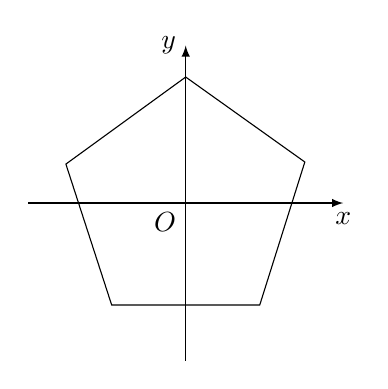
\begin{tikzpicture}[>=latex]
\draw [->] (-2,0) -- (2,0) node [below] {$x$};
\draw [->] (0,-2) -- (0,2) node [left] {$y$};
\draw (0,0) node [below left] {$O$};
\draw (90:1.6) -- (162:1.6) -- (234:1.6) -- (306:1.6) -- (379:1.6) -- cycle;
\end{tikzpicture}
\end{center}
\item 画一个底面边长是$3\text{cm}$、高是$4.5\text{cm}$的正三棱柱的直观图.
\item 已知正六棱锥的底面边长为$6\text{cm}$, 高为$15\text{cm}$. 画它的直观图, 比例尺为$1:3$.
\item 如图, 点$A$在平面$\alpha$上, 点$BC$在平面$\beta$上, 平面$\alpha$与平面$\beta$相交于直线$l$, 画出过点$ABC$的平面与平面$\alpha \beta$的交线.
\begin{center}
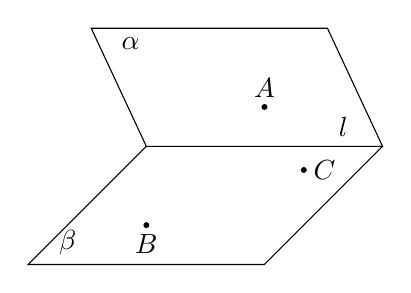
\begin{tikzpicture}[>=latex]
\draw (0,0) -- (3,0) -- (2.3,1.5) --++ (-3,0) -- cycle;
\draw (2.5,0) node [above] {$l$} (-0.2,1.5) node [below] {$\alpha$}; 
\filldraw (1.5,0.5) circle (0.03) node [above] {$A$};
\draw (0,0) --++ (-1.5,-1.5) --++ (3,0) -- (3,0);
\draw (-1,-1.5) node [above] {$\beta$};
\filldraw (0,-1) circle (0.03) node [below] {$B$} (2,-0.3) circle (0.03) node [right] {$C$};
\end{tikzpicture}
\end{center}
\item 如图, 已知正方体$ABCD-A_1B_1C_1D_1$, 点$E$是棱$DC$的中点.
\begin{center}
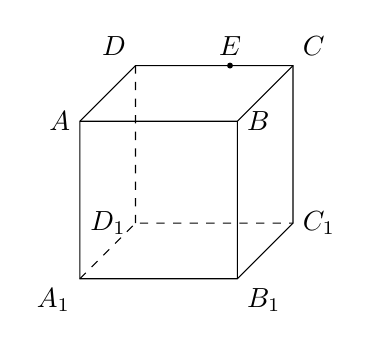
\begin{tikzpicture}[>=latex]
\draw (0,0) node [below left] {$A_1$} coordinate (A) --++ (2,0) node [below right] {$B_1$} coordinate (B) --++ (45:{2/2}) node [right] {$C_1$} coordinate (C)
--++ (0,2) node [above right] {$C$} coordinate (C1)
--++ (-2,0) node [above left] {$D$} coordinate (D1) --++ (225:{2/2}) node [left] {$A$} coordinate (A1) -- cycle;
\draw (A) ++ (2,2) node [right] {$B$} coordinate (B1) -- (B) (B1) --++ (45:{2/2}) (B1) --++ (-2,0);
\draw [dashed] (A) --++ (45:{2/2}) node [left] {$D_1$} coordinate (D) --++ (2,0) (D) --++ (0,2);
\filldraw ($(C1)!0.4!(D1)$) circle (0.03) node [above] {$E$};
\end{tikzpicture}
\end{center}
(1) 画出由点$EAB_1$确定的平面$\alpha$截正方体所得的截面;\\
(2) 平面$\alpha$将正方体分割成两个多面体, 画出这两个多面体的直观图.
\item 用厚纸做一个正四棱锥的模型.
\item 将一个直三棱柱分割成三个三棱锥, 试将这三个三棱锥分离, 并画出这些三棱锥的直观图.
\item 圆柱体、圆锥体的母线和旋转轴的位置关系如何?
\item 从一个底面半径和高都是$R$的圆柱中, 挖去一个以圆柱的上底为底、下底面的中心为顶点的圆锥, 得到一个如图所示的几何体. 如果用一个与圆柱下底面距离等于$d$并且平行于底面的平面去截这个几何体. 求截面面积.
\begin{center}
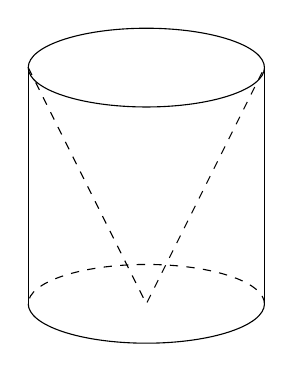
\begin{tikzpicture}[>=latex]
\draw (0,0) ellipse (1.5 and 0.5);
\draw (-1.5,0) --++ (0,-3) (1.5,0) --++ (0,-3);
\draw (-1.5,-3) arc (180:360:1.5 and 0.5);
\draw [dashed] (1.5,-3) arc (0:180:1.5 and 0.5) (-1.5,0) -- (0,-3) -- (1.5,0);
\end{tikzpicture}
\end{center}
\item 如果球的大圆面积增为原来的$100$倍, 那么球的半径有什么变化?
\item 已知$OA$是球$O$的半径, $OA=5$, $O_2$是$OA$上的两点, 平面$\alpha$、$\beta$分别通过点$O_2$, 且垂直于$OA$, 截得圆$O_1$和圆$O_2$, 当圆$O_1$、圆$O_2$的面积分别为$9$$\pi$、$21\pi$时, 求$O_1O_2$的长.
\begin{center}
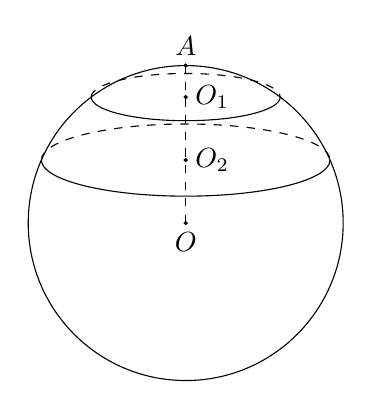
\begin{tikzpicture}[>=latex,scale = 0.4]
\filldraw (0,0) circle (0.05) node [below] {$O$};
\filldraw (0,5) circle (0.05) node [above] {$A$};
\filldraw (0,2) circle (0.05) node [right] {$O_2$};
\filldraw (0,4) circle (0.05) node [right] {$O_1$};
\draw (0,0) circle (5);
\draw [dashed] ({-sqrt(21)},2) arc (180:0:{sqrt(21)} and {sqrt(21)/4});
\draw ({-sqrt(21)},2) arc (180:360:{sqrt(21)} and {sqrt(21)/4});
\draw [dashed] (-3,4) arc (180:0:3 and {3/4});
\draw (-3,4) arc (180:360:3 and {3/4});
\draw [dashed] (0,0) -- (0,5);
\end{tikzpicture}
\end{center}
\item 用一块正方形的厚纸板, 以它的一个顶点为圆心、边长为半径画弧, 沿弧剪下一个扇形, 试用这块扇形厚纸板制作一个圆锥筒.
\item 经过球面上不同两点的大圆有多少个? 并说明理由.
\item 已知正三棱锥的底面边长是$2$, 高是$4$, 求该正三棱锥的表面积.
\item 已知直四棱柱的底面是边长分别为$5\text{cm}$、$6\text{cm}$.且有一条对角线长为$8\text{cm}$的平行四边形, 该四棱柱最长的对角线为$10\text{cm}$, 求该四棱柱的侧面积.
\item 已知侧面积为$27$的正三棱柱的侧棱恰好是某个圆柱的三条母线, 且这个圆柱的底面半径为$2$, 求这个圆柱的表面积.
\item 如图, 已知一个圆锥的底面半径为$2$, 高为$2$, 且在这个圆锥中有一个高为$x$的圆柱.\\
(1) 写出此圆柱的侧面积表达式;\\
(2) 当$x$为何值时, 此圆柱的侧面积最大?
\begin{center}
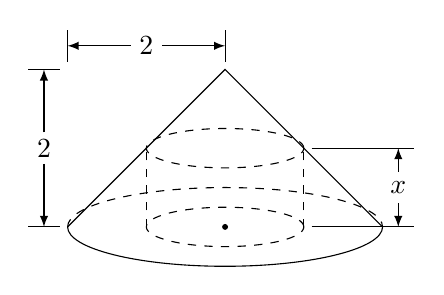
\begin{tikzpicture}[>=latex]
\filldraw (0,0) circle (0.03);
\draw [dashed] (0,0) ellipse (1 and 0.25);
\draw [dashed] (0,1) ellipse (1 and 0.25);
\draw [dashed] (-1,0) -- (-1,1) (1,0) -- (1,1);
\draw [dashed] (-2,0) arc (180:0:2 and 0.5);
\draw (-2,0) arc (180:360:2 and 0.5);
\draw (-2,0) -- (0,2) -- (2,0);
\draw (1.1,0) -- (2.4,0) (1.1,1) -- (2.4,1);
\draw [->] (2.2,0.3) -- (2.2,0);
\draw [->] (2.2,0.7) -- (2.2,1);
\draw (2.2,0.5) node {$x$};
\draw (0,2.1) -- (0,2.5) (-2,2.1) -- (-2,2.5);
\draw [->] (-1.2,2.3) -- (-2,2.3);
\draw [->] (-0.8,2.3) -- (0,2.3);
\draw (-1,2.3) node {$2$};
\draw (-2.1,0) -- (-2.5,0) (-2.1,2) -- (-2.5,2);
\draw [->] (-2.3,1.2) -- (-2.3,2);
\draw [->] (-2.3,0.8) -- (-2.3,0);
\draw (-2.3,1) node {$2$};
\end{tikzpicture}
\end{center}
\item 已知三棱柱的底面是$\triangle ABC$, $AB=13\text{cm}$, $BC=5\text{cm}$, $CA=12\text{cm}$, 侧棱$AA'$的长是$20\text{cm}$, 且侧棱$AA'$与底面所成的角为$60^\circ$, 求这个三棱柱的体积.
\item 在万吨水压机上, 有四根圆柱形钢柱, 高$18$米, 内径$0.4$米, 外径$1$米, 求这四根钢柱的质量(结果精确到$1$吨, 钢的密度为$7.9$克/立方厘米).
\item 已知正三棱锥的侧棱长为$10$厘米, 侧棱与底面所成的角等于$\arcsin \dfrac 35$, 求这个三棱锥的体积.
\item 一块正方形薄铁板的边长是$22$厘米, 以它的一个顶点为圆心、边长为半径画弧, 沿弧剪下一个扇形, 用这块扇形铁板围成一个圆锥筒, 求它的容积(结果精确到$1$立方厘米).
\item 已知三个球的表面积之比是$1:2:3$, 求这三个球的体积之比.
\item 有一堆相同规格的六角螺帽毛坯共重$5.8$千克, 已知每个六角螺帽毛坯的底面六边形的边长是$12$毫米, 高$10$毫米, 内孔直径是$10$毫米, 共有毛坯多少个(铁的密度为$7.8$克/立方厘米)?
\item 已知正六棱柱最长的一条对角线长为$13$厘米, 侧面积为$180$平方厘米, 求这个棱柱的体积.
\item 有一个铜制工件, 它的下部分呈正四棱柱形, 上部分呈正四棱锥形, 且这个正四棱锥以正四棱柱的上底为底, 已知正四棱柱的底面边长是$50$毫米, 高是$10$毫米, 正四棱锥的侧面呈正三角形, 这个工件的质量是多少千克(结果精确到$0.1$千克, 铜的密度是$8.9$克/立方厘米)?
\item 有一个空心钢球, 重$142$克, 测得外径等于$5$厘米, 求它的内径. (结果精确到$0.1$厘米, 钢的密度为$7.9$克/立方厘米)
\item 已知香港的位置为东经$114^\circ 10'$, 北纬$22^\circ 18'$, 江西井冈山的位置为东经$114^\circ 10'$, 北纬$26^\circ 34'$, 求这两个城市之间的距离. (地球半径约为$6371$千米, 结果精确到$1$千米)
\item 在北纬$60^\circ$圈上有甲乙两地, 它们的纬度圈上的弧长等于$\dfrac{\pi R}2$($R$是地球的半径), 求甲乙两地的球面距离.
\item 在北纬$45^\circ$圈上有甲乙两地. 经度相差$90^\circ$, 求甲乙两地的球面距离与地球半径的比.
\item 纬度为$\alpha$的纬度圈上有甲乙两地, 它们的纬度圈上的弧长等于$\pi R\cos \alpha$($R$是地球的半径), 求甲乙两地的球面距离.
\item 地球上有甲乙两个城市, 甲在北纬$30^\circ$, 东经$83^\circ$, 乙在北纬$30^\circ$, 西经$97^\circ$, 求过这两个城市在纬度圈上的距离与它们在地球表面上的球面距离的比.
\item 判断下列说法是否正确, 如果正确, 请说明理由; 如果不正确, 请举一个反例.\\
(1) 直四棱柱是长方体;\\
(2) 侧棱长相等, 且底面是正多边形的棱锥是正棱锥;\\
(3) 各侧面都是正三角形的四棱锥是正四棱锥;\\
(4) ``三条侧棱两两互相垂直, 且侧棱与底面所成角都相等''是``棱锥为正三棱锥''的充要条件.
\item 现有以下三个命题: \textcircled{1} 底面是平行四边形的四棱柱是平行六面体; \textcircled{2} 底面是矩形的平行六面体是长方体; \textcircled{3} 直四棱柱是直平行六面体. 其中真命题的序号是\blank{50}.
\item 选择题:
如果一个三棱锥的底面是直角三角形, 那么这个三棱锥的三个侧面\bracket{20}
\twoch{都不是直角三角形}{至多只能有一个是直角三角形}{至多只能有两个是直角三角形}{可能都是直角三角形}
\item 已知棱锥的侧棱与底面所成的角都相等, 试说出棱锥的顶点在底面内的射影所在的位置, 并证明你的结论.
\item 已知棱锥的顶点在底面内的射影在底面的内部, 其侧面与底面所成的角都相等, 试说出棱锥的顶点在底面内的射影所在的位置, 并证明你的结论.
\item 已知正方体$ABCD-A_1B_1C_1D_1$的棱长为$2$.
\begin{center}
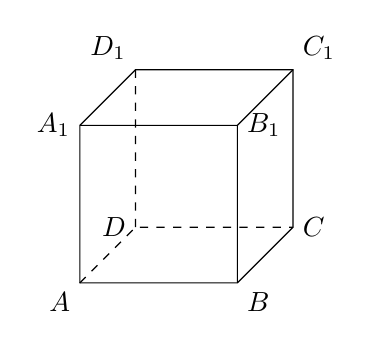
\begin{tikzpicture}[>=latex]
\draw (0,0) node [below left] {$A$} coordinate (A) --++ (2,0) node [below right] {$B$} coordinate (B) --++ (45:{2/2}) node [right] {$C$} coordinate (C)
--++ (0,2) node [above right] {$C_1$} coordinate (C1)
--++ (-2,0) node [above left] {$D_1$} coordinate (D1) --++ (225:{2/2}) node [left] {$A_1$} coordinate (A1) -- cycle;
\draw (A) ++ (2,2) node [right] {$B_1$} coordinate (B1) -- (B) (B1) --++ (45:{2/2}) (B1) --++ (-2,0);
\draw [dashed] (A) --++ (45:{2/2}) node [left] {$D$} coordinate (D) --++ (2,0) (D) --++ (0,2);
\end{tikzpicture}
\end{center}
(1) 平面$DCB_1A_1$, 将正方体分割成两个多面体, 作出这两个多面体, 并说出它们的几何体;\\
(2) 平面$AB_1C_1$将直三棱柱$ABC-A_1B_1C_1$分制成两个多面体, 作出这两个多面体, 并说出它们是怎样的几何体.
\item 已知长方体的长为$\sqrt {29}$, 长、宽、高之和为$9$, 求这个长方体的表面积.
\item 已知一个长方体的长、宽、高的比为$1: 2: 3$, 对角线长是$2\sqrt {14}$, 求这个长方体的体积.
\item 已知正方体$ABCD-A'B'C'D'$的边长为$a$, 点$E,F$分别是棱$AD,AB$的中点;\\
(1) 求证: 四边形$EFB'D'$是等腰梯形;\\
(2) 求等腰梯形$EFB'D'$的面积.
\item 已知一个圆锥的高是$10\text{cm}$, 侧面展开图是半圆, 求这个圆锥的侧面积.
\item 已知电镀螺杆的尺寸如图所示(单位: 毫米). 如果每平方米用锌$0.11$千克, 那么要电镀$100$个这样的螺杆需要多少锌?
\begin{center}
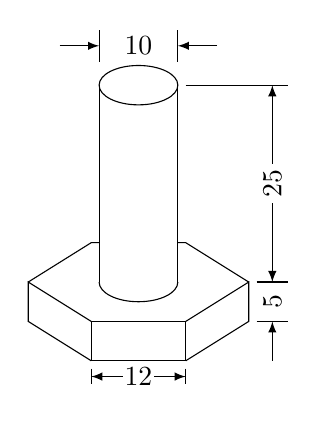
\begin{tikzpicture}[>=latex, scale = 0.1]
\draw (-6,0) -- (6,0) -- (6,5) -- (-6,5) -- cycle;
\draw (6,5) --++ (8,5) --++ (0,-5) -- (6,0);
\draw (-6,5) --++ (-8,5) coordinate (T) --++ (0,-5) -- (-6,0);
\draw (T) --++ (8,5) --++ (12,0) --++ (8,-5);
\draw (T) ++ (14,0) coordinate (O);
\filldraw [white] (O) ++ (5,0) rectangle++ (-10,25);
\draw (O) ++ (5,0) --++ (0,25);
\draw (O) ++ (-5,0) --++ (0,25);
\draw (O) ++ (5,0) arc (0:-180:5 and 2.5);
\draw (O) ++ (0,25) ellipse (5 and 2.5);
\draw (-6,-1) -- (-6,-3) (6,-1) -- (6,-3);
\draw [->] (-2,-2) -- (-6,-2);
\draw [->] (2,-2) -- (6,-2);
\draw (0,-2) node {$12$};
\draw (15,5) -- (19,5) (15,10) -- (19,10);
\draw (17,7.5) node {\rotatebox{90}{$5$}};
\draw [->] (17,0) -- (17,5);
\draw [->] (17,20) -- (17,10);
\draw [->] (17,25) -- (17,35);
\draw (6,35) -- (19,35);
\draw (17,22.5) node {\rotatebox{90}{$25$}};
\draw (-5,38) -- (-5,42) (5,38) -- (5,42);
\draw [->] (-10,40) -- (-5,40);
\draw [->] (10,40) -- (5,40);
\draw (0,40) node {$10$}; 
\end{tikzpicture}
\end{center}
\item 已知一个球的大圆的周长是$80$厘米, 求这个球的表面积.
\item 已知地球的半径约是$6371$米, 火星直径约是地球直径的一半, 地球和火星的体积各是多少?
\item 已知一个直角三角形的两条直角边分别为$15$厘米、$20$厘米, 以它的斜边为旋转轴旋转一周得旋转体, 求旋转体的体积.
\item 海面上地球球心角$1'$所对的大圆弧长约为$1$海里, $1$海里约是多少千米? (地球的半径约是$6371$千米)
\item 在半径是$r$的球面上, 有两点$AB$, 半径$OA$和$OB$的夹角是$n^\circ (n<180) $求$AB$的两点的球面距离.
\item 已知长方体$ABCD-A_1B_1C_1D_1$的高为$h$, 底面积为$P$, 对角面$BB_1D_1D$的面积为$Q$.
求它的侧面积.
\item 已知圆柱$A$和圆锥$B$的底面直径和高都与球$C$的直径相等, 求证: 圆柱$A$、球$C$、圆锥$B$的体积的比是$3: 2: 1$.
\item 在赤道上, 东经$140^\circ$上有点$A$, 西经$130^\circ$上有点$B$, 求$AB$两点的球面距离(地球半径约为$6371$千米).
\item 设$AB$是球$O$的直径, $AB=50$, $O_1,O_2$是$AB$上的两点, 平面$\alpha, \beta$分别通过点$O_1,O_2$, 且垂直于$AB$截得圆$O_1$圆$O_2$, 当圆$O_1$圆$O_2$的面积分别为$49\pi$、$400\pi$时, 求$O_1,O_2$两点的距离.
\item 有一块长为$a$、宽为$b$($a>b$)的矩形木板, 将木板的一边着地, 另外相对的两边紧贴在垂直于地面且二面为直角的墙角的两面上, 围出一个三棱柱的谷仓, 应怎样围才能使谷仓的面积最大?
\item 一种旅行包上的号码锁有三个拨号盘, 每个拨号盘上有从$0$到$9$的$10$个数字, 这三个拨号盘可组成多少种不同的三位数号码?
\item 一个商场共有$9$个出入口, 若某人在进出商场时不要走同一个出入口, 则他一次进出商场共有多少种不同的进出法?
\item 已知$a\in \{1,3,5,7\}$, $b\in \{2,4,6,8\}$, 在平面直角坐标系中, 直线方程$ax+by+1=0$可以表示多少条直线?
\item 为了提高产品质量控制生产过程的温度、材料处理的时间和添加剂的剂量, 为此工厂进行生产试验. 试验控制温度有$150^\circ\text{C}$、$160^\circ\text{C}$和$170^\circ\text{C}$三种, 材料处理的时间有$10$分钟、$12$分钟两种, 添加剂的剂量有$2$克, $4$克和$6$克三种, 共需要做多少次试验?
\item $(a_1+a_2+a_3)(b_1+b_2+b_3+b_4)(c_1+c_2)$展开后共有多少项?
\item 某个学校食堂准备了$5$种素菜、$3$种荤菜和$3$种汤, 取一种素菜、一种荤菜、一种汤配成一套菜, 这个学校食堂可以有多少套不同的菜?
\item 用$1$、$2$、$3$、$4$、$5$这五个数字可以组成多少个无重复数字的三位数的奇数?
\item 要把$4$封信投入$3$个信箱, 共有多少种不同的投法? (允许将信全部或部分投入某一个信箱)
\item 用$0$、$1$、$2$、$3$、$4$、$5$这六个数字可以组成多少个数字不重复的三位数?
\item 用$0$、$1$、$2$、$3$、$4$、$5$这六个数字可以组成多少个三位数?
\item 已知集合$M=\{-3,-2,-1,0,1,2\}$, 点$P(a,b) $在直角坐标平面上, 且$a, b\in M$.\\
(1) 平面上共有多少个满足条件的点$P$?\\
(2) 有多少个点$P$在第二象限内?\\
(3) 有多少个点$P$不在直线$y=x$上?
\item 从$15$件不同的礼品中取出$4$件分送给$4$个学生, 共有多少种不同的送法?
\item 从$5$名运动员中选出$3$名参加乒乓球团体比赛, 并排定他们的出场顺序, 有多少种不同的方法?
\item 从若干种不同的盆景中选出$2$种摆放在阳台的左右两侧, 如果想要有$30$种不同的选法, 那么最少要准备多少种不同的盆景?
\item 从$2,3,4,5,7,11$这六个数字中选出$2$个数字作为分子和分母, 共能组成多少个大小不同的分数?
\item 从$6$名志愿者中选出$4$人分别从事翻译、导游、导购、保洁工作, 其中甲、乙两人不能从事翻译工作, 选派志愿者的方案共有多少种?
\item 求下列各式中$n$($n\in \mathbf{N}^*$)的值.\\
(1) $\mathrm{P}_{2n}^3=11\mathrm{P}_n^3$;\\
(2) $\mathrm{P}_n^5+\mathrm{P}_n^4=4\mathrm{P}_n^3$;\\
(3) $\mathrm{P}_n^3=n\mathrm{P}_3^3$.
\item 用$1$、$2$、$3$、$4$、$5$、$6$能组成多少个没有重复数字且大于$500$的三位数?
\item 用$1$、$2$、$3$、$4$、$5$、$6$能组成多少个没有重复数字且小于$500$的三位数?
\item 已知$\mathrm{P}_{10}^m=10\times 9\times \cdots \times 5$, 求正整数$m$的值.
\item 从$6$名学生中任选$3$人分别担任语文、数学、英语课代表, 其中学生甲不能担任数学课代表, 共有多少种不同的选法?
\item $5$名学生站成一排, 其中甲学生不能站在排头的不同站法有多少种?
\item $4$名教师、$3$名男生、$2$名女生排成一排, 要求$3$名男生排在一起, $2$名女生排在一起, 共有多少种不同的排队方法?
\item 用$0$、$1$、$2$、$3$、$4$、$5$这六个数字可以组成多少个没有重复数字的四位奇数?
\item 用$0$到$9$这十个数可以组成多少个没有重复数字的四位数?
\item 已知甲、乙、丙等$7$人站成一排, 求分别按下列要求排队各有多少种不同的排法;\\
(1) 甲、乙都与丙相邻;\\
(2) 甲、乙之间有且只有$1$人.
\item 化简: $\dfrac 1{2!}+\dfrac 2{3!}+\dfrac 3{4!}+\cdots +\dfrac{n-1}n$($n\in \mathbf{N}^*$, $n\ge 2$). 
\item 已知抛物线方程为$y=ax^2+bx+c$, 集合$M=\{-2,-1,0,1,2,3,4\}$, $a,b,c\in M$, 且$a,b,c$两两不相等, 满足条件的抛物线中, 过原点的抛物线有多少条?
\item 求证: $\mathrm{P}_1^1+2\mathrm{P}_2^2+3\mathrm{P}_3^3+\cdots +n\mathrm{P}_n^n=\mathrm{P}_{n+1}^{n+1}-1$($n\in \mathbf{N}^*$).
\item 乒乓球队的$10$名队员中有$3$名主力队员, 派$5$名队员参加比赛, 其中, $3$名主力队员要安排在第一、三、五位置, 其余$7$名队员中的$2$名要安排在第二、四位置, 共有多少种不同的安排方法?
\item 用$0$、$6$、$8$这三个数字可组成多少个没有重复数字的整数?
\item 用$0$到$9$这十个数字可组成多少个能被$5$整除的无重复数字的二位数?
\item 某班的新年联欢会原定的$5$个节目已排成节目单, 开始演出前又增加了$2$个新节目, 如果将这两个新节目插入原节目单中, 那么有多少种不同的插法?
\item 用$0$到$9$这十个数字, 可组成多少个没有重复数字的四位数的偶数?
\item 有$A,B,C,D,E$五列火车停在某车站并行的$5$条火车轨道上, 如果快车$A$不能停在第$3$道上, 慢车$B$不能停在第$1$道上, 那么这五列火车的停车方法有多少种?
\item 某班级周一的课表要排入政治、语文、数学、物理、化学、体育共$6$门学科, 如果第一节课不排体育课, 最后一节课不排数学课, 那么共有多少种不同的排法?
\item 用$0$到$5$这六个数字可组成无重复数字的四位数的偶数, 且这个偶数的百位、十位上都是奇数, 满足条件的数共有多少个?
\item 将$8$个相同的小球放入编号为$1$、$2$、$3$的三个盒内, 要求每个盒子的球数不小于它的编号数, 共有多少种不同的放法?
\item 用$1$、$2$、$3$、$4$、$5$可组成多少个无重复数字且比$13245$大的五位数?
\item 试确定下列问题是排列问题还是组合问题.\\
(1) $3$本不同的书借给甲、乙、丙$3$名学生, 每人$1$本, 有多少种不同的借法?\\
(2) 从$10$本书中任意取$5$本赠送给$1$名学生, 有多少种不同的送法?\\
(3) 从$15$人中选$3$人去参加数学竞赛, 有多少种不同的选法?\\
(4) 从$15$人中选$3$人分别参加数学、物理、化学竞赛, 有多少种不同的选法?
\item 某项测试共有两组试题. 要求从第一组$10$个问题中选择$8$个, 从第二组$5$个问题中选择$4$个, 要完成这项测试有多少种不同的选择试题的方法?
\item 已知$100$件产品中有$2$件次品如果从这些产品中任取$5$件, 那么其中恰好有$2$件次品的取法有多少种?
\item 某班级共有$25$名团员, 其中$10$名男团员, $15$名女团员.\\
(1) 如果从中推选$2$名男团员和$3$名女团员参加团代会, 那么有多少种不同的推选方法?\\
(2) 如果从中推选$2$名男团员和$3$名女团员组成团支部分别担任不同职务, 那么有多少种不同的推选方法?
\item 以某个圆周上的$10$个点为顶点, 可以作多少个三角形?
\item 求下列各式中$n$($n\in \mathbf{N}^*$)的值:\\
(1) $\mathrm{C}_n^5+\mathrm{C}_n^6=\mathrm{C}_{n+1}^3$;\\
(2) $\mathrm{C}_{n+1}^{n-1}=\dfrac 7{15}\mathrm{P}_{n+1}^3$.
\item 求证: $\mathrm{C}_n^m=\dfrac{m+1}{n+1}\mathrm{C}_{n+1}^{m+1}$($n,m\in \mathbf{N}^*$, $n\ge m$).
\item 计算: $\mathrm{C}_3^0+\mathrm{C}_4^1+\mathrm{C}_5^2+\cdots +\mathrm{C}_{20}^7$.
\item 从$8$名男运动员与$7$名女运动员中选出$5$名男运动员与$5$名女运动员组成一个运动队, 不同的选法共有多少种?
\item 要从$6$名男学生与$6$名女学生中选出$2$名男学生与$2$名女学生组成一个学习小组, 共有多少种不同的选法?
\item 已知平面上共有$10$个点, 其中有$4$个点在一条直线上, 除此之外再没有三点共线, 以这$10$个点为顶点能组成多少不同的三角形?
\item (1) 计算$\mathrm{C}_2^0+\mathrm{C}_2^1+\mathrm{C}_2^2$;\\
(2) 计算: $\mathrm{C}_3^0+\mathrm{C}_3^1+\mathrm{C}_3^2+\mathrm{C}_3^3$;\\
(3) 猜想$\mathrm{C}_n^0+\mathrm{C}_n^1+\mathrm{C}_n^2+\cdots +\mathrm{C}_n^{n-1}+\mathrm{C}_n^n(n\in \mathbf{N}^*) $的值, 并证明你的结果;\\
(4) 你能否利用第(3)题来求一个集合的子集的个数? 为什么?
\item 用一组$5$条平行线与另一组$4$条平行线共可围成多少个平行四边形?
\item 已知$\dfrac{\mathrm{C}_{2n}^{n-1}}{\mathrm{C}_2^n(n-1)}=\dfrac{56}{15}$, 求正整数$n$的值.
\item 从$3$本不同的语文书、$4$本不同的数学书和$3$本不同的物理书中取出$4$本书, 且要求三种书都有共有多少种不同的取法?
\item 从$5$名女学生和$4$名男学生中选出$4$人担任$4$种不同的工作, 且要求选出的$4$人中男女学生都有, 共有多少种不同的选法?
\item 已知集合$AB$都含有$12$个元素, $A\cap B$含有$4$个元素, 集合$C$含有$3$个元素, 且$C\subsetneqq A\cup B,C\cap B\ne \varnothing$, 求满足条件的集合$C$的个数.
\item 某旅游团要从$8$个风景点中选$2$个风景点作为当天的旅游地, 求分别满足以下条件的选法的种数.\\
(1) 甲乙风景中至少选一个;\\
(2) 甲乙风景点中至多选一个;\\
(3) 甲乙风景点中必须选一个, 而且只能选一个.
\item 用二项式定理展开下列两式:\\
(1) $(a+2b)^6$;\\
(2) $(1-\dfrac 1x)^5$.
\item 化简:\\
(1) $(1+\sqrt x)^5+(1-\sqrt x)^5$;\\
(2) $(2x+y)^4-(2x-y)^4$.
\item (1) 求$(x-1)^{15}$的二项展开式中的前$4$项;\\
(2) 求$(2a^3-3b^2)^{10}$的二项展开式中的第$8$项.
\item 求下列各式的二项展开式中指定的项的系数:\\
(1) $(1-\dfrac 1{2x})^{10}$二项展开式中含$\dfrac 1{x^4}$的项;\\
(2) $(3x^3-\dfrac 1{3x^3})^{10}$的二项展开式中的常数项.
\item 在$(3x-2y)^9$的展开式中, 求二项式系数的和以及各项系数的和.
\item (1) 用二项式定理证明: $(n+1)^n-1$能被$n^2$整除;\\
(2) 用二项式定理证明: $99^{10}-1$能被$1000$整除.
\item 已知$(1+x)^n$的二项展开式中第$4$项与第$8$项的二项系数相等, 求这两项的二项式系数.
\item 求证: $2^n-\mathrm{C}_n^1\cdot 2^{n-1}+\mathrm{C}_n^2\cdot 2^{n-2}+\cdots +\mathrm{C}_n^{n-1}\cdot 2+(-1)^n=1$.
\item $\mathrm{C}_n^1+3\mathrm{C}_n^2+9\mathrm{C}_n^3+\cdots +3^{n-1}\mathrm{C}_n^n$等于\bracket{20}.
\fourch{$4^n$}{$\dfrac{4^n}3$}{$\dfrac{4^n}3-1$}{$\dfrac{4^n-1}3$}
\item 已知$n$为大于$1$的自然数, 证明: $(1+\dfrac 1n)^n>2$.
\item 在$(x^2-\dfrac 3x)^n$的二项展开式中, 有且只有第五项的二项式系数最大, 求$\mathrm{C}_n^0-\dfrac 12\mathrm{C}_n^1+\dfrac 14\mathrm{C}_n^2-\cdots +(-1)^n\cdot \dfrac 12\mathrm{C}_n^n$.
\item 选择题:
$\mathrm{C}_{100}^0-\mathrm{C}_{100}^2+\mathrm{C}_{100}^4-\cdots +\mathrm{C}_{100}^{98}+\mathrm{C}_{100}^{100}$等于\bracket{20}.
\fourch{$-2^{50}$}{$0$}{$1$}{$2^{50}$}
\item 求$(\dfrac{\sqrt x}2-\dfrac 2{\sqrt x})^{10}$的二项展开式的中间一项.
\item 求$(x\sqrt y-y\sqrt x)^{11}$的二项展开式的中间两项.
\item 在$(1+3x)^n$的二项展开式中, 末三项的二项式系数之和等于$631$.\\
(1) 求二项展开式中二项式系数最大的项是第几项;\\
(2) 求二项展开式中系数最大的项.
\item 求$77^{77}-15$除以$19$的余数.
\item 求证: $2^{6n-3}+3^{2n-1}$能被$11$整除.
\item 已知$(x+1)^n=x^n+\cdots +ax^3+bx^2+cx+1$($n\in \mathbf{N}^*$), 且$a:b=3:1$, 求$c$的值.
\item 某学生要从$2$本科技书、$2$本政治书和$3$本文艺书中任取一本书, 共有\blank{50}种不同的取法.
\item 如果将$3$名男学生与$2$名女学生排成一排, 且$2$名女生不排在相邻位置上, 那么不同排法的种数是\blank{50}.
\item 计划在某画廊展出$10$幅不同的画, 其中$1$幅为水彩画, $4$幅为油画, $5$幅为国画, 排成一行陈列, 如果同一品种的画必须排在一起, 并且水彩不能排在两端, 那么陈列方式有	\blank{50}种.
\item 用数字$0$、$1$、$2$、$3$、$4$、$5$可组成没有重复数字的六位数, 其中数字$2$、$4$排在相邻数位上, 满足条件的六位数共有\blank{50}个.
\item $(x^2-\dfrac 1{2\sqrt x})^3$的二项展开式的第$3$项是\blank{50}.
\item 若把$4$只不同颜色的球放人$3$个不同的袋内, 则不同的放法的种数是\bracket{20}.
\fourch{$4^3$}{$3^4$}{$\mathrm{P}_4^3$}{$\mathrm{C}_4^3$}
\item 若$\mathrm{C}_n^3=12\mathrm{P}_n^1$, 则$n$的值为\bracket{20}.
\fourch{$3$}{$5$}{$7$}{$10$}
\item 语文兴趣小组有学生$10$人, 从中选派$3$人参加诗歌朗诵会, 不同的选派方法的种数是\bracket{20}.
\fourch{$720$}{$360$}{$240$}{$120$}
\item 用$1$、$2$、$3$、$4$、$5$这五个数字可以组成比$20000$大, 且百位数不是$3$的没有重复数字的五位数, 满足条件的五位数共有\bracket{20}.
\fourch{$96$个}{$78$个}{$77$个}{$64$个}
\item 某市工商局会同商检局对$35$种商品进行抽样检查, 鉴定结果为其中有$5$种是不合格商品, 现从这$35$种商品中任取$3$种, 至少有$2$种不合格商品的取法种数是\bracket{20}.
\fourch{$\mathrm{C}_5^3+\mathrm{C}_5^2\mathrm{C}_{30}^1$}{$\mathrm{P}_5^3+\mathrm{P}_5^2\mathrm{P}_{30}^1$}{$\mathrm{C}_5^2\mathrm{C}_{30}^1$}{$\mathrm{P}_5^2\mathrm{P}_{30}^1$}
\item $(x-1)^n$的二项展开式中第$m$项($m\le n$, $n\in \mathbf{N}^*$)的二项式的系数是\bracket{20}.
\fourch{$\mathrm{C}_n^{m-1}$}{$(-1)^{m-1}\mathrm{C}_n^m$}{$\mathrm{C}_n^m$}{$(-1)^m\mathrm{C}_n^m$}
\item 某学生邀请$10$位同学中的$6$位参加一个生日聚会, 其中$2$位同学要么都邀请, 要么都不邀请, 共有多少种邀请方法?
\item 某次篮球赛预赛分成$3$个赛区进行, 第一赛区男队、女队各$9$队, 第二赛区男队、女队各$10$队, 第三赛区男队$9$队, 女队$10$队, 各赛区男队、女队各取前$4$名参加决赛. 预赛、决赛都采用单循环制比赛, 一共需要进行多少场比赛?
\item 已知$(x\sin \theta +1)^6$的二项展开式$x^2$项的系数与$(x-\dfrac{15}2\cos \theta)^4$的二项展开式中$x^3$项的系数相等, 求$\cos \theta$的值.
\item 关于$x$的方程$\mathrm{C}_{34}^{x^2-2x}=\mathrm{C}_{34}^{5x-6}$的解集是\blank{50}.
\item $6$个人排成一列, 其中甲乙两人之间至少有两个人的不同排法种数是\blank{50}.
\item 由数字$1$、$2$、$3$、$4$组成没有重复数字的不同自然数的个数是\blank{50}.
\item 若$m\in \{2,5,7,8\}$, $n\in\{1,3,4,6\}$, 则方程$\dfrac{x^2}m+\dfrac{y^2}n=1$表示焦点在$x$轴上的椭圆有\blank{50}个.
\item 若$(1+\sqrt x)^n$的展开式的系数和大于$8$且小于$32$, 则系数最大的项是\blank{50}.
\item 已知在$100$件产品中有$3$件是次品, 如果从中任意抽取$5$件, 那么其中至多有$2$件次品的抽法的种数是\bracket{20}.
\fourch{$\mathrm{C}_3^2\mathrm{C}_{97}^3$}{$\mathrm{C}_{100}^5\mathrm{C}_3^2$}{$\mathrm{C}_{100}^5\mathrm{C}_3^2\mathrm{C}_{97}^2$}{$\mathrm{C}_3^2\mathrm{C}_{97}^2+\mathrm{C}_3^1\mathrm{C}_{97}^4$}
\item 从$10$名男学生和$12$名女学生中各选$3$名排成一列, 其中男、女相间排成一列的不同排法的种数是\bracket{20}.
\fourch{$2\mathrm{P}_{10}^3\mathrm{P}_{12}^3$}{$\mathrm{P}_{10}^3\mathrm{P}_{12}^3$}{$\mathrm{C}_4^3\mathrm{P}_{10}^3\mathrm{P}_{12}^3$ }{$\mathrm{P}_4^3\mathrm{P}_{10}^3\mathrm{P}_{12}^3$}
\item $100$件产品中有$97$件合格品与$3$件次品, 从中任意抽取$7$件进行检查;\\
(1) 抽出的$7$件都是合格品的抽法有多少种?\\
(2) 抽出的$7$件恰好有$2$件是次品的抽法有多少种?\\
(3) 抽出的$7$件至少有$2$件是次品的抽法有多少种?
\item 求$\mathrm{C}_{10}^1+2\mathrm{C}_{10}^2+4\mathrm{C}_{10}^3+\cdots +2^9\mathrm{C}_{10}^{10}$的值.
\item 已知$(2^{\lg x}-1)^n$的二项展开式中, 最后三项的二项式系数和等于$22$, 中间项为$-1280$, 求$x$的值.
\item 判断下列现象哪些是随机现象, 哪些不是随机现象;\\
(1) 月球绕着地球转, 地球绕着太阳转;\\
(2) 气压低的地方, 水的沸点低;\\
(3) 黄浦江水位超出警戒线$1$米.
\item 袋中有$10$个球, 记有号码$0$、$1$、$2$、$3$、$4$、$5$、$6$、$7$、$8$、9. 求下列事件的概率:\\
(1) 任意取出$2$个球, 号码为$1$、$2$;\\
(2) 任意取出$3$个球, 没有号码$3$.
\item 掷两颗骰子, 求出现下列事件的概率;\\
(1) 两颗骰子的点数之和等于$2$;\\
(2) 两颗骰子的点数之和等于$3$;\\
(3) 两颗骰子的点数之和等于$5$;\\
(4) 两颗骰子的点数之和等于$7$.
\item 已知某班有$38$名学生, 小李、小王、小张是该班的$3$名学生, 某次班会决定随机地挑选这$3$名学生在会上发言, 求下列事件出现的概率;\\
(1) 小李、小王、小张按此次序被选中;\\
(2) 小李、小王、小张按任意次序被选中.
\item 某剧场将举办$8$场音乐会. 其中$2$场演奏莫扎特的作品, 小方对 $8$场音乐会都很感兴趣, 难于选择, 最后决定用抽签的方法决定参加哪两场音乐会. 小方抽到两场都是莫扎特音乐会的概率是多少? 两场中$1$场是莫扎特音乐会的概率是多少?
\item 一部$4$卷的文集, 按任意次序放到书架上, 求各卷自左向右或自右向左的卷号为$1$、$2$、$3$、$4$的概率.
\item 已知$10$个产品中有$3$个次品, 从中任取$5$个, 求至少有一个次品的概率.
\item 某种密码由$8$个数字组成, 且每个数字可以是$0$、$1$、$2$、…、$9$中的任意一个数, 求这种密码由完全不同的数字组成的概率.
\item 一工厂生产的$10$个产品中有$9$个一等品、$1$个二等品, 现从这批产品中抽取$4$个, 求其中恰好有一个二等品的概率.
\item 掷一颗骰子, 求出现点数不小于$2$的概率.
\item 某城镇共有$10000$辆自行车, 牌照编号从$00001$到$10000$, 求在此城镇中偶然遇到的一辆自行车, 其牌照号码中有数字$8$概率.
\item 近代数学家掷硬币试验的一些结果列于下表:
\begin{center}
\begin{tabular}{|c|c|c|}
\hline
试验者 & 掷硬币次数$n$ & 正面出现次数$m$\\ \hline
德·摩尔根 & $2048$ & $1061$\\ \hline
蒲丰 & $4040$ & $2048$\\ \hline
皮尔逊 & $12000$ & $6019$\\ \hline
皮尔逊 & $24000$ & $12012$\\ \hline
维尼 & $30000$ & $14994$\\ \hline
\end{tabular}
\end{center}
分别求正面出现的频率, 并根据这些结果说一说前人所做掷硬币试验反映了怎样的规律.
\item 两台机床加工同样的零件, 第一台出现废品的经验概率是$0.03$, 第二台出现废品的经验概率是$0.02$, 加工出来的零件放在一起, 并且已知第一台加工的零件比第二台加工的零件多一倍, 求任意取出的零件是合格品的经验概率.
\item 在某城市中共发行甲、乙、丙三种报纸, 在这个城市的居民中, 订甲报的人占总人数的$45\%$, 订乙报的人占$35\%$, 订丙报的人占$30\%$, 同时订甲乙两报的人占$10\%$, 同时订甲丙两报的人占$8\%$, 同时订乙丙两报的人占$5\%$, 同时订三种报纸的人占$3\%$, 求:\\
(1) 只订甲报的人所占百分比;\\
(2) 只订甲报或乙报的人所占百分比;\\
(3) 只订一种报纸的人所占百分比;\\
(4) 正好订两种报纸的人所占百分比;\\
(5) 至少订一种报纸的人所占百分比;\\
(6) 不订任何报纸的人所占百分比.
\item 将$n$间房间分给$n$个人, 每个人都以相等的可能性进入每一间房间. 而且每间房间里的人数没有限制, 求不出现空房的概率.
\item 把$10$本书随机地排在书架上, 求其中指定的$3$本书排在一起的概率.
\item 某人有$5$把钥匙, 但只有一把能打开门, 他每次取一把钥匙尝试开门, 求试到第$3$把钥匙时才打开门的概率.
\item 某次测验有$10$道备用试题, 甲同学在这$10$道题中能够答对$6$题, 现在备用试题中随机抽考$5$题, 规定答对$4$题或$5$题为优秀, 答对$3$题为及格;\\
(1) 求甲同学获优秀的概率;\\
(2) 求甲同学至少能够及格的概率.
\item 某中学有十八个班级, 每班选出三个代表出席学生代表会议, 从$54$名代表中任选$18$名组成工作委员会, 分别求下列事件的概率:\\
(1) 高一(1)班在工作委员会中有代表;\\
(2) 每个班级在工作委员会中都有代表.
\item $4$个人每人带一件礼品参加聚会, 聚会开始后, 先把$4$件礼品编号, 然后每个人任抽一个号码, 按号领取礼品, 求这$4$个人都没拿到自己带去的礼品的概率.
\item 一批零件中有$9$个合格品和$3$个废品, 安装机器时, 从这批零件中随机取出一个, 如果每次取出的成品不放回去, 分别求在取得第$1$件合格品以前已取出$x$件废品数的概率, $x=0,1,2,3$.
\item 已知血型为$O,A,B,AB$型的概率分别为$0.46$、$0.40$、$0.11$、$0.03$. 任意抽取一人, 求下列事件的概率:
(1) 抽出人为$O$型血的概率;\\
(2) 抽出人为$A$或$B$型血的概率;\\
(3) 抽出人不是$AB$型血的概率.
\item 从一个有$800$户居民的小区中抽取一个$30$户的样本, 样本中每户的人数如下所示: $5$、$6$、$3$、$3$、$2$、$3$、$3$、$3$、$4$、$4$、$3$、$2$、$7$、$4$、$3$、$5$、$4$、$4$、$3$、$3$、$4$、$3$、$3$、$1$、$2$、$4$、$3$、$4$、$2$、$4$;\\
(1) 估计该小区平均每户的人数;\\
(2) 估计该小区居民总数.
\item 人们常认为$16^\circ\text{C}$是宜人的年平均温度, 单纯根据平均气温的报告来选择野营地点是否恰当? 为什么?
\item 某校教师进行体格检查, 测得他们的收缩压(单位: 毫水汞柱)的值如下表所示:
\begin{center}
\begin{tabular}{|c|c|c|c|c|c|c|}
    \hline
    收缩压范围 & $89.5-104.4$ & $104.5-119.4$ & $119.5-134.4$ & $134.5-149.4$ & $149.5-164.4$ & $164.5-179.4$\\ \hline
    人数 & $24$ & $62$ & $72$ & $26$ & $12$ & $4$\\ \hline
\end{tabular}
\end{center}
(1) 求该校教师收缩压的平均数和中位数;(用各收缩压范围的中点的值代表该范围的取值, 结果精确到$0.1$);\\
(2) 作出收缩压分布频率直方图.
\item 某计算机操作培训班各学员的考试成绩如下表所示:
\begin{center}
\begin{tabular}{|c|c|c|c|c|c|c|c|c|}
\hline
得分 & $100$ & $90$ & $80$ & $70$ & $67$ & $65$ & $63$ & $55$\\ \hline
人数 & $2$ & $3$ & $10$ & $25$ & $13$ & $3$ & $2$ & $2$\\ \hline
\end{tabular}
\end{center}
求学员考试成绩的平均数、中位数和得分的方差.
\item 利用``随机数表'', 从$1$到$100$的数字中, 随机抽取$10$个数字作样本.
\item 从$2$开始的$200$个偶数, 即$2$、$4$、$6$、$8$、$\cdots$、$400$中, 用系统抽样的办法抽取$20$个偶数作样本.
\item 如果采用分层抽样, 从个体数为$N$的总体中抽取一个容量为$n$的样本, 那么每个个体的样本, 被抽到的概率等于\blank{50}.
\item 在下列问题中, 各采用怎样的抽样方法抽取样本较为合适?\\
(1) 从$20$台手提电脑中抽取$4$台进行质量检查;\\
(2) 某大剧院共有$80$排座位, 每排共有$120$个座位, 座位号为1-120, 有一次音乐会坐满了观众, 音乐会结束后为听取观众意见需留下$80$名观众进行座谈;\\
(3) 某学校共有七个年级$1600$名学生, 其中, 六年级学生$160$名, 七年级学生$160$名, 八年级学生$240$名, 九年级学生$240$名, 高中一年级学生$200$名, 高中二年级学生$280$名, 高中三年级学生$320$名, 从中抽取一个容量为$160$的样本.
\item 某学校共有$2000$名学生, 从中选取$20$名学生参加学生代表大会, 试采用随机抽样和分层抽样两种方法进行具体实施.
\item 某学校学生志愿者协会共有$250$名成员, 其中高中一年级学生$88$名, 高中二年级学生$112$名, 高中三年级学生$50$名, 为了了解志愿者活动与学校学习之间的关系, 需要抽取$50$名学生进行调查, 试确定抽取方法并写出过程.
\item 从某中学$200$名新生中随机抽取$10$名进行身高测量, 得数据为: $168$、 $159$、$166$、$163$、$170$、$161$、$167$、$155$、$162$、$169$(单位: $\text{cm}$). 试估计该中学$200$名新生的平均身和高于$165\text{cm}$的概率估计值.
\item 某班级有$40$名同学参加打靶训练, 他们的成绩如下表所示(单位: 环):
\begin{center}
\begin{tabular}{|c|c|}
    \hline
    检验成绩 & 频数 \\ \hline
    $4$、$5$ &$2$\\ \hline
    $5$、$6$&$3$\\ \hline
    $6$、$7$&$10$\\ \hline
    $7$、$8$&$15$\\ \hline
    $8$、$9$&$8$\\ \hline
    $9$、$10$&$2$  \\ \hline
\end{tabular}
\end{center}
求该班同学的成绩和$2\sigma$区间估计.
\item 某校一年级共有学生$220$名, 为了解该校高一学生的生长情况, 决定做一次抽样调查, 按随机抽样方法抽$22$名学生, 测量他们的身高体重记录在下表中, 表中$h$(单位: 米)表示学生的身高, $g$(单位: 千克)是学生的体重.
\begin{center}
    \begin{tabular}{|c|c|c|c|c|c|c|c|c|}
        \hline
        $h$ & $1.57$ & $1.65$ & $1.56$ & $1.67$ & $1.55$ & $1.71$ & $1.77$ & $1.77$\\ \hline
        $g$ & $44$ & $53$ & $46$ & $50$ & $43$ & $57$ & $60$ & $66$\\ \hline
        $h$ & $1.60$ & $1.65$ & $1.62$ & $1.70$ & $1.58$ & $1.73$ & $1.80$ & $1.80$\\ \hline
        $g$ & $47$ & $55$ & $49$ & $59$ & $52$ & $61$ & $67$ & $72$\\ \hline
        $h$ & $1.50$ & $1.55$ & $1.62$ & $1.64$ & $1.59$ & $1.60$ &  & \\ \hline
        $g$ & $41$ & $42$ & $51$ & $51$ & $54$ & $57$ &  & \\ \hline
    \end{tabular}
\end{center}
求该校高中一学生总体体重均值的点估计值, 总体身高均值的点估计值及总体体重均值的$2\sigma$区间估计.
\item 为了检测某种产品的质量, 抽取了一个容量为$100$的样本, 测得它们的质量如下表所示:
\begin{center}
    \begin{tabular}{|c|c|}
        \hline
        质量区间 & 频数 \\ \hline
        $(10.75, 10.85)$ & $3$ \\ \hline
        $(10.85, 10.95)$ & $9$ \\ \hline
        $(10.95, 11.05)$ & $13$ \\ \hline
        $(11.05, 11.15)$ & $16$ \\ \hline
        $(11.15, 11.25)$ & $26$ \\ \hline
        $(11.25, 11.35)$ & $20$ \\ \hline
        $(11.35, 11.45)$ & $7$\\ \hline
        $(11.45, 11.55)$ & $4$\\ \hline
        $(11.55, 11.65)$ & $2$\\ \hline
    \end{tabular}
\end{center}
求该种产品的质量$2\sigma$区间估计.
\item 某公司为了解员工的年收入情况, 随机抽取$10$名员工, 调查他们的年收入如下: $81000$、$77000$、$69000$、$77000$、$83000$、$100000$、$62000$、$77000$、$58000$、$91000$(单位: 元), 请据此估计该公司员工年平均收入、年中等收入和年收入众数.
\item 为考察某校高中三年级男学生的身高, 随机地抽取$50$名男学生, 测得他们的身高(单位: $\text{cm}$)如下表所示:
\begin{center}
    \begin{tabular}{|c|c|c|c|c|c|c|c|c|c|}
        \hline
        $170$ & $170$ & $165$ & $169$ & $167$ & $167$ & $170$ & $161$ & $164$ & $167$\\ \hline
        $171$ & $163$ & $163$ & $169$ & $166$ & $168$ & $168$ & $165$ & $160$ & $168$\\ \hline
        $158$ & $160$ & $163$ & $167$ & $173$ & $168$ & $169$ & $170$ & $160$ & $164$\\ \hline
        $171$ & $169$ & $167$ & $159$ & $151$ & $168$ & $170$ & $174$ & $160$ & $168$\\ \hline
        $176$ & $157$ & $162$ & $166$ & $158$ & $164$ & $180$ & $179$ & $169$ & $169$\\ \hline
    \end{tabular}
\end{center}
(1) 填写下表:
\begin{center}
    \begin{tabular}{|c|c|c|}
        \hline
        身高 & 频数 & 频率$f$ \\ \hline
        $[150.5,153.5)$ &&\\ \hline		
        $[153.5,156.5)$	&&\\ \hline
        $[156.5,159.5)$	&& \\ \hline
        $[159.5,162.5)$	&& \\ \hline
        $[162.5,165.5)$	&& \\ \hline
        $[165.5,168.5)$	&& \\ \hline
        $[168.5,171.5)$	&& \\ \hline
        $[171.5,174.5)$	&& \\ \hline
        $[174.5,177.5)$	&& \\ \hline
        $[177.5,180.5)$ && \\ \hline
    \end{tabular}
\end{center}	
(2) 估计该校高中三年级学生的平均身高;\\
(3) 画出该校高中三年级学生身高的频率直方图, 分析该校高中三年级学生身高的分布情况.
\item 某区教育局为了了解初中学生的作业负担, 随机抽查了$25$个初中学生, 调查他们平均每天在家庭作业上所花的时间, 结果如下表所示(单位: 分):
\begin{center}
    \begin{tabular}{|c|c|c|c|c|}
        \hline
        $40$ & $80$ & $80$ & $90$ & $90$\\ \hline
        $50$ & $90$ & $90$ & $100$ & $110$\\ \hline
        $70$ & $70$ & $80$ & $70$ & $80$\\ \hline
        $40$ & $80$ & $70$ & $50$ & $70$\\ \hline
        $60$ & $50$ & $100$ & $80$ & $90$\\ \hline
    \end{tabular}
\end{center}
求出该区初中学生家庭作业时间的平均数、中位数, 并画出频率直方图来描述这些数据.
\item 研究$40$个妇女的血液中含钾的数据(单位: 毫克/升), 记录如下:
\begin{center}
    \begin{tabular}{|c|c|c|c|c|}
        \hline
        $3.2$ & $4.9$ & $3.8$ & $3.6$ & $3.4$\\ \hline
        $5.8$ & $5.3$ & $4.6$ & $5.1$ & $3.6$\\ \hline
        $6.0$ & $4.7$ & $4.3$ & $4.2$ & $4.4$\\ \hline
        $4.5$ & $5.0$ & $4.4$ & $5.8$ & $3.9$\\ \hline
        $4.2$ & $3.9$ & $3.8$ & $3.7$ & $4.2$\\ \hline
        $4.3$ & $4.9$ & $5.6$ & $3.7$ & $4.1$\\ \hline
        $2.7$ & $4.0$ & $4.2$ & $4.3$ & $4.3$\\ \hline
        $5.1$ & $5.2$ & $4.7$ & $4.5$ & $4.9$\\ \hline
    \end{tabular}
\end{center}
求含钾量的平均数、中位数、标准差, 并画出分成$7$个组的含钾量的频率直方图.
\item 抽烟对健康有害. 调查$20$个肺部患病的病人每天抽烟的数量(单位: 支), 如下表所示:
\begin{center}
    \begin{tabular}{|c|c|c|c|c|}
        \hline
        $10$ & $22$ & $11$ & $13$ & $0$\\ \hline
        $8$ & $13$ & $9$ & $12$ & $11$\\ \hline
        $0$ & $17$ & $18$ & $15$ & $16$\\ \hline
        $14$ & $19$ & $14$ & $0$ & $11$\\ \hline
    \end{tabular}
\end{center}
分$6$组画出抽烟分布频率直方图.
\item 什么是样本的代表性?
\item 从某批灯泡中随机抽取$10$只作寿命实验, 其寿命(单位: 时)如下: $1050$、$1100$、$1120$、$1280$、$1250$、$1040$、$1030$、$1110$、$1240$、$1300$, 求该批灯泡寿命的平均数和标准差.
\item 某学校共有$1000$名学生, 其中高中一年级有学生$300$名, 高中二年级有学生$300$名, 高中三年级有学生$400$名, 为调查学生日均上网时间, 需要$100$名学生参加调查, 试选取合适的抽样方法并实施.
\item 仓库内有$36$个货架, 随机抽取$10$个货架, 这$10$个货架上的货物的价值(单位: 元)分别为$540$、$290$、$610$、$380$、$510$、$580$、$610$、$560$、$770$、$600$. 试估计仓库内货物的总价值.
\item 某校有$200$名学生参与研究性学习, 每人参加一个课题组的研究, 其中参加文学类的有$33$人, 参加理化类的有$30$人, 数学类的有$62$人, 参加社会科学类的有$47$人, 参加信息类的有$28$人.\\
(1) 列出学生参加各类课题组的分布表;\\
(2) 画出学生参加各类课题组的频率直方图.
\item 利用随机投点法求抛物线$y=x^2-4$与$x$轴组成的封闭图形的面积.
\item 用集合语言表示下列语句, 并画图表示: 点$P$在直线$l$上, 点$P$不在平面$\alpha$上, 直线$l$与平面$\alpha$相交于$O$;\\
\item 用集合语言表述下图中空间的点、直线和平面的关系.
\begin{center}
    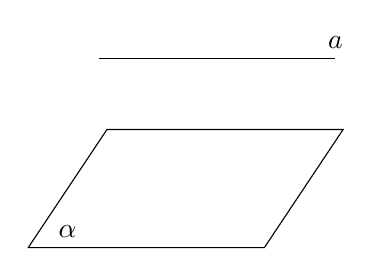
\begin{tikzpicture}
        \draw (0,0) -- (3,0) -- (4,1.5) -- (1,1.5) -- cycle;
        \draw (0.5,0) node [above] {$\alpha$};
        \draw (0.9,2.4) -- (3.9,2.4) node [above] {$a$}; 
    \end{tikzpicture}
    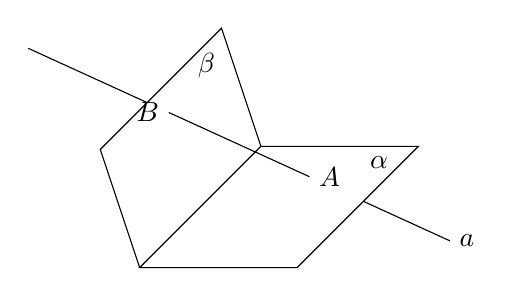
\begin{tikzpicture}
        \draw [name path = alpha] (0,0,0) -- (2,0,0) -- (2,0,-4)  -- (0,0,-4) -- cycle;
        \draw (1.5,0,-4) node [below] {$\alpha$};
        \draw [name path = beta] (0,0,0) -- (-0.5,1.5,0) -- (-0.5,1.5,-4)  -- (0,0,-4);
        \draw (-0.5,1.5,-3.5) node [below] {$\beta$};
        \draw (1,0,-3) node [right] {$A$} coordinate (A);
        \draw (-0.4,1.2,-2) node [left] {$B$} coordinate (B);
        \draw (A) -- (B);
        \path [name path = line1] ($(A)!-1!(B)$) coordinate (C) -- (A);
        \path [name path = line2] ($(B)!-1!(A)$) coordinate (D) -- (B);
        \path [name intersections = {of = line1 and alpha, by = S}];
        \draw (S) -- (C) node [right] {$a$};
        \path [name intersections = {of = line2 and beta, by = T}];
        \draw (T) -- (D);
    \end{tikzpicture}
\end{center}
\item 判断下列说法是否正确, 如果正确, 请说明依据; 如果不正确, 请举反例.\\
(1) 梯形是平面图形;\\
(2) 三点可确定一个平面;\\
(3) 四边相等的四边形是菱形.
\item 如图所示, 正方体$ABCD-A_1B_1C_1D_1$,的棱长为$a$, $ E,F,E_1,F_1$分别为棱的中点.
\begin{center}
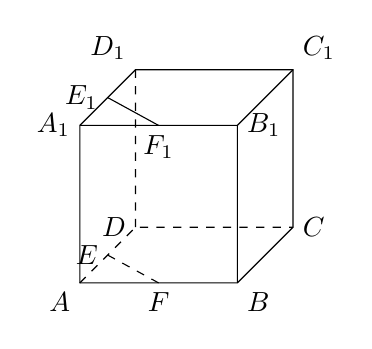
\begin{tikzpicture}[>=latex]
\draw (0,0) node [below left] {$A$} coordinate (A) --++ (2,0) node [below right] {$B$} coordinate (B) --++ (45:{2/2}) node [right] {$C$} coordinate (C)
--++ (0,2) node [above right] {$C_1$} coordinate (C1)
--++ (-2,0) node [above left] {$D_1$} coordinate (D1) --++ (225:{2/2}) node [left] {$A_1$} coordinate (A1) -- cycle;
\draw (A) ++ (2,2) node [right] {$B_1$} coordinate (B1) -- (B) (B1) --++ (45:{2/2}) (B1) --++ (-2,0);
\draw [dashed] (A) --++ (45:{2/2}) node [left] {$D$} coordinate (D) --++ (2,0) (D) --++ (0,2);
\draw [dashed] ($(A)!0.5!(D)$) node [left] {$E$} -- ($(A)!0.5!(B)$) node [below] {$F$};
\draw ($(A1)!0.5!(D1)$) node [left] {$E_1$} -- ($(A1)!0.5!(B1)$) node [below] {$F_1$};
\end{tikzpicture}
\end{center}
(1) 求证: $\angle AFE=\angle A_1F_1E_1$;\\
(2) 求异面直线$EF$与$CD$所成的角的大小.
\item 已知直线$a,b$和平面$\alpha$所成的角均为$30^\circ$, 能否判断$a\parallel b$? 为什么?
\item 已知$ABCD-A_1B_1C_1D_1$为正方体.
\begin{center}
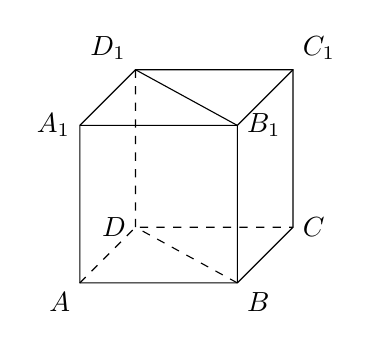
\begin{tikzpicture}[>=latex]
\draw (0,0) node [below left] {$A$} coordinate (A) --++ (2,0) node [below right] {$B$} coordinate (B) --++ (45:{2/2}) node [right] {$C$} coordinate (C)
--++ (0,2) node [above right] {$C_1$} coordinate (C1)
--++ (-2,0) node [above left] {$D_1$} coordinate (D1) --++ (225:{2/2}) node [left] {$A_1$} coordinate (A1) -- cycle;
\draw (A) ++ (2,2) node [right] {$B_1$} coordinate (B1) -- (B) (B1) --++ (45:{2/2}) (B1) --++ (-2,0);
\draw [dashed] (A) --++ (45:{2/2}) node [left] {$D$} coordinate (D) --++ (2,0) (D) --++ (0,2);
\draw [dashed] (B) -- (D);
\draw (B1) -- (D1);
\end{tikzpicture}
\end{center}
(1) 求二面角$A_1-D_1D-B_1$的大小;\\
(2) 求二面角$A-B_1D_1-C$的大小.
\item 作正三棱锥$P-ABC$的直观图, 使它的高为$3\text{cm}$. 底边长为$4\text{cm}$.
\item 在球内有相距$9\text{cm}$的两个平行的截面. 若两截面圆为球的小圆时, 其面积分别为$49\pi \text{cm}^2$、$400\pi \text{cm}^2$, 求此球的表面积及体积.
\item 已知圆锥的母线$l$与底面成$45^\circ$角, 这个圆锥的体积为$9\pi \text{cm}^3$, 求这个圆锥的高$h$及侧面积.
\item 已知正三棱锥的底边长为$1$, 侧棱长为$2$, 求这个正三棱锥的体积.
\item 设地球半径为$R$, 城市$A$位于东经$90^\circ$, 北纬$60^\circ$, 城市$B$位于东经$150^\circ$、北纬$60^\circ$, 求城市$AB$之间的距离.
\item 有$4$名同学选报铅球、跳高、跳远三个体育项目, 如果每三个报一项, 那么共有多少种报名方法?
\item 从$6$种菜品种中选出$3$种, 分别种植在不同的$3$块地上进行试验, 有多少种不同的种植方法?
\item 已知$\dfrac 1{\mathrm{C}_5^n}-\dfrac 1{\mathrm{C}_6^n}=\dfrac 7{10\mathrm{C}_7^n}$, $n\in \mathbf{N}^*$, 求$\mathrm{C}_8^n$;\\
\item 已知$\mathrm{P}_m^2=7\mathrm{P}_{m-4}^2$, $m\in \mathbf{N}^*$, 求$m$的值.
\item 已知$(x\sqrt x-\dfrac 1x)^4$的二项展开式的第$5$项为$\dfrac{15}2$, 求$\displaystyle\lim_{n\to\infty}(x^{-1}+x^{-2}+\cdots +x^{-n}) $的值.
\item 设$n\in \mathbf{N}^*$, 求证: $\mathrm{C}_n^1+\mathrm{C}_n^2+\cdots +\mathrm{C}_n^n=1+2+2^2+\cdots +2^{n-1}$.
\item 某人参加某抽奖活动, 现有$300$张抽奖劵, 其中有$1$个一等奖, $2$个二等奖, $3$个三等奖, 求这个人抽一次奖就中奖的概率.
\item 在一个袋内装有同样大小、同样质地的红球$5$只, 黑球$4$只, 白球$2$只, 绿球$1$只, 今从袋中任意摸取一个球;\\
(1) 摸出红球或黑球的概率;\\
(2) 摸出红球或黑球或白球的概率.
\item 求$(1.009)^5$的近似值\blank{50}(结果精确到$0.001$).
\item 设球的半径为$4$, 用一个平面截球, 使截面圆的半径为$2$, 则截面与球心的距离\blank{50}.
\item $4$名男生、$4$名女生站站成一排, 男女间隔排列, 则不同的排法有\blank{50}种.
\item 已知长方体$ABCD-A_1B_1C_1D_1$中, $AB=BC=4$, $AA_1=2$.
\begin{center}
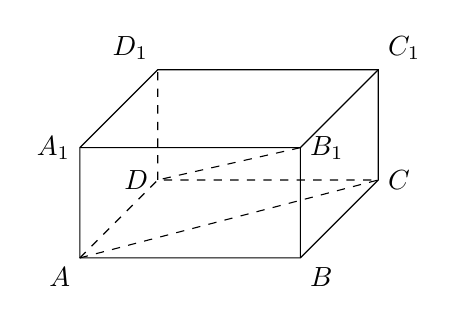
\begin{tikzpicture}[>=latex,scale = 0.7]
\draw (0,0) node [below left] {$A$} coordinate (A) --++ (4,0) node [below right] {$B$} coordinate (B) --++ (45:{4/2}) node [right] {$C$} coordinate (C)
--++ (0,2) node [above right] {$C_1$} coordinate (C1)
--++ (-4,0) node [above left] {$D_1$} coordinate (D1) --++ (225:{4/2}) node [left] {$A_1$} coordinate (A1) -- cycle;
\draw (A) ++ (4,2) node [right] {$B_1$} coordinate (B1) -- (B) (B1) --++ (45:{4/2}) (B1) --++ (-4,0);
\draw [dashed] (A) --++ (45:{4/2}) node [left] {$D$} coordinate (D) --++ (4,0) (D) --++ (0,2);
\draw [dashed] (B1) -- (D) (A) -- (C);
\end{tikzpicture}
\end{center}
(1) 求异面直线$B_1C_1$与$AC$所成的角的大小及距离;\\
(2) 求异面直线$AA_1$所$B_1D$所成角的大小及距离.
\item 在正方体$ABCD-A_1B_1C_1D_1$中, $AB=2\sqrt 2$, $BD$与$AC$交于点$O$.\\
(1) 求直线$D_1O$与平面$ABCD$所成角的正弦值;\\
(2) 求点$D$到平面$ACD_1$的距离.
\item 已知圆柱的轴截面$ABCD$是正方形, 点$E$在底面圆周上, $AF\perp DE$, $F$是垂足;\\
(1) 求证: $AF\perp DB$;\\
(2) 如果圆柱与三棱锥$D-ABE$的体积比等于$3\pi$, 求直线$DE$与平面$ABCD$所成的角的正切值.
\item 一个球受热膨胀, 如果它的表面积增加$21\%$. 那么这个球的半径增加多少?
\item 求$\mathrm{C}_{3\pi }^{38-n}+\mathrm{C}_{21+n}^{3\pi }$($n\in \mathbf{N}^*$)的值.
\item 利用二项式定理证明: $3^n>2^{n-1}(n+2)$($n\in \mathbf{N}^*$, $n\ge 2$).
\item 以一个正方体的顶点为顶点能组成多少个三棱锥?
\item 已知$(\sqrt[3]x-\dfrac 1{\sqrt x})^n$的二项展开式中, 第三项与第二项的二项式系数之比为$11:2$ , 求正整数$n$及二项展开式中的所有的有理项.
\item 已知$(x^{\lg x}+1)^n$的二项展开式中, 求三项的二项式系数的和为22. 二项式系数最大的项为20000, 求实数$x$的值.
\item 从$3$名男生和$n$名女生中, 任意选$3$人参加会议, 已知选出的$3$人中至少有一名女生的概率是$\dfrac{34}{35}$, 求$n$的值.
\item 某造于为了估计自己的射击技术, 一天内连续进行$50$次射击, 命中环数记录如下:
\begin{center}
    \begin{tabular}{|c|c|c|c|c|c|c|c|c|c|}
        \hline
        $10$ & $5$ & $5$ & $8$ & $7$ & $8$ & $6$ & $9$ & $7$ & $8$\\ \hline
        $6$ & $6$ & $5$ & $6$ & $7$ & $8$ & $10$ & $9$ & $7$ & $8$\\ \hline
        $8$ & $7$ & $6$ & $5$ & $9$ & $9$ & $7$ & $8$ & $8$ & $5$\\ \hline
        $8$ & $6$ & $7$ & $6$ & $9$ & $6$ & $9$ & $8$ & $8$ & $6$\\ \hline
        $7$ & $6$ & $8$ & $10$ & $7$ & $10$ & $8$ & $7$ & $7$ & $9$\\ \hline
    \end{tabular}
\end{center}
(1) 求该选手这一天平均一次命中的环数及标准差;\\
(2) 求该选手均值的$\sigma$区间估计.
\item 用随机投点法, 求$y=\sin x(0\le x\le \pi) $与$x$轴组成的封闭图形的面积.


\end{enumerate}

\end{document}